%% =====================================================================
%%  X-UAD : A Unified, Uncertainty-Aware and Self-Explaining Detector for
%%          Physical and Digital Face Attacks   (revision 2)
%%  IEEE conference format (IEEEtran).  Compile with pdflatex + bibtex:
%%     pdflatex xuad_v2 && bibtex xuad_v2 && pdflatex xuad_v2 && pdflatex xuad_v2
%%  Prose follows the revised draft; figures and supplementary tables are
%%  restored from xuad.tex; every number is \input from tables/ (generated by
%%  scripts/make_tables.py from results/*.json).
%% =====================================================================
\documentclass[conference]{IEEEtran}
\IEEEoverridecommandlockouts

\usepackage{cite}
\usepackage{amsmath,amssymb,amsfonts}
\usepackage{graphicx}
\usepackage{booktabs}
\usepackage{multirow}
\usepackage{xcolor}
\usepackage{textcomp}
\usepackage{url}
\usepackage[hidelinks]{hyperref}

\newcommand{\bs}[1]{\boldsymbol{#1}}
\newcommand{\R}{\mathbb{R}}
\newcommand{\ket}[1]{\lvert #1 \rangle}
\newcommand{\bra}[1]{\langle #1 \rvert}
\newcommand{\braket}[2]{\langle #1 \vert #2 \rangle}

\begin{document}

\title{X-UAD: A Unified, Uncertainty-Aware and Self-Explaining Detector for
Physical and Digital Face Attacks}

\author{}

\maketitle

\begin{abstract}
Face recognition systems can be defeated by presentation attacks staged in front
of the camera, such as a printed photograph, a replayed video or a silicone mask,
and by digital manipulation of the captured image through face swapping,
expression reenactment, synthesis or adversarial perturbation. A detector built for
one family is usually blind to the other, and the recent unified detectors that
handle both still share three practical weaknesses. They emit a single uncalibrated
score with no way of signalling that an input resembles nothing they were trained
on; they cannot point to where in the frame the evidence sits; and when they do
explain themselves, the explanation comes from a language model that never observed
the detector's internal state. We present X-UAD, one model aimed at all three.
Adaptive Quantum Attention adds a Born-rule scoring channel beside ordinary
dot-product attention. It is sign-invariant by construction, which matches the
interference character of moir\'e, halftone and checkerboard evidence, and it costs
$\mathcal{O}(dL)$ parameters rather than $\mathcal{O}(d^{2})$. The same learnable
rotations define an orthonormal evidence basis whose measurements serve
simultaneously as classification features and, completely unchanged, as the
explanation shown to a reader. A decoupled evidential head predicts class direction
and evidence magnitude separately, and pseudo-unseen evidence suppression trains
that magnitude on blends of two attack families, an outlier proxy built from the
attack taxonomy itself. On a difficulty-calibrated, identity-disjoint benchmark of
eight attack families with pixel-level ground truth, X-UAD reaches $1.46\%$ ACER
against $0.71\%$ for the strongest baseline, while giving the best calibration among
the working detectors ($1.94\%$ ECE) and the best evidence localisation ($77.8\%$
region-level IoU). On attack families withheld from training it achieves the
highest average detection rate ($77.5\%$), and the synthetic-blend objective alone
is worth $5.4$ AUROC points on the uncertainty channel. We also report, without
softening it, that every method in the comparison collapses under a serious change
of capture domain, and that all results come from a single seed on a simulated
benchmark. Code, the benchmark generator and configuration files mapping the same
pipeline onto public capture-based datasets are released.
\end{abstract}

\begin{IEEEkeywords}
face anti-spoofing, presentation attack detection, deepfake detection, unified
attack detection, vision transformer, quantum-inspired attention, evidential deep
learning, uncertainty estimation, open-set recognition, explainable AI
\end{IEEEkeywords}

% =====================================================================
\section{Introduction}
% =====================================================================
Consider everything that can go wrong in front of a face-unlock camera. Someone
could hold up a printed photo of you. They could replay a video of your face on a
phone screen. They could wear a silicone mask shaped like your face. These are
\emph{physical} attacks, and each leaves a physical fingerprint behind: the halftone
dot pattern of a printer, the pixel grid of a phone screen aliasing into a moir\'e
pattern, the waxy sheen and flattened texture of silicone.

Now consider what can go wrong \emph{after} the camera has captured a real,
unmanipulated photograph. Someone could swap in a different identity. They could
drive your expression with someone else's performance. They could generate a face
that never belonged to any real person. They could add a barely visible pattern of
noise that flips a classifier's decision without a human noticing anything at all.
These are \emph{digital} attacks, and their fingerprints look entirely different:
blending seams where a swapped face meets the original, resolution mismatches,
checkerboard patterns left behind by the upsampling layers of a generator, unusual
peaks in the frequency spectrum.

Because these two sets of fingerprints look nothing alike, the two research
communities that study them grew up separately. Face anti-spoofing work focused on
texture and depth cues \cite{liu2018auxiliary,yu2020cdcn,yu2021revisiting,wang2022ssan}.
Face forgery research focused on frequency artifacts and blending cues
\cite{rossler2019ff,li2020celebdf,frank2020frequency,wang2020cnnspot}. The split is
understandable, but it is not something you can deploy. An operator needs one
decision, one threshold and one audit trail, not two models that might disagree
with no principled way to combine them. A recent line of work
\cite{yu2024unified,yuan2024challenge,ma2025uniattackplus,chen2025uniattack,zhang2024unidefense}
has finally built unified corpora and joint detectors that handle both attack
families at once, which is real progress. It also exposed a problem that had been
hiding underneath. On the attack types these models were trained on they are
essentially saturated, with ACER around $0.5$ to $1.4\%$, but the moment you hold out
an attack family during training and show it only at test time, error rates jump to
between $22$ and $44\%$ with large variance between runs \cite{yu2024unified}.
Unified detection, in other words, is solved in-distribution and still wide open
out-of-distribution.

Layered on top of that gap, we see three capabilities missing from almost all of
this literature, and all three are things an operator genuinely needs the moment a
score comes back ambiguous rather than obviously fake or obviously real.

The first is a real notion of \emph{not knowing}. A softmax output is fundamentally
a closed-set quantity, since it has to redistribute all of its probability mass
across the classes it was trained on. A completely novel kind of attack therefore
gets assigned high confidence toward whichever known class it happens to resemble
most. What is actually needed is a second-order belief, one that is allowed to sit
close to empty when the input does not look like anything the model has learned.

The second is \emph{evidence localisation}. Depth-map supervision
\cite{liu2018auxiliary,yu2021revisiting} works reasonably for physical attacks,
since a printed photo or a replayed video really is flatter than a real face. But
depth is a proxy for liveness rather than a map of forensic evidence, and it says
nothing useful about a digitally swapped face that came from a perfectly live,
perfectly three-dimensional original capture.

The third is an \emph{explanation that is actually tied to the decision}. Recent
work has started feeding face images into multimodal language models and asking
them to describe what looks fake \cite{huang2024ffaa,guo2025m2f2det}. The results
read fluently, but the language model never sees the detector's internal state. It
is reasoning over the raw image, independently of whatever the classifier actually
computed. Its narrative is therefore correlated with the decision at best, and it
is free to mention artifacts such as ``a visible screen bezel'' that are not
actually present in the frame or that the detector never used.

\subsection{What this paper does}
We built X-UAD, a single model that detects physical and digital face attacks
together, reports how much it does not know, points to where the evidence is, and
explains its own decision in language that traces back to numbers it actually
computed. Three ideas make this work.

\textbf{Adaptive Quantum Attention (AQA).} Ordinary attention scores a pair of
tokens with an unbounded linear functional, the dot product. A great deal of the
evidence for face attacks, though, is fundamentally an interference phenomenon: a
moir\'e beat, a checkerboard pattern, a spectral peak. These show up in the
\emph{squared magnitude} of a projection, not in the raw projection, and their sign
carries no information. A moir\'e fringe and its photographic negative are the same
evidence, but a dot product treats them as opposites. AQA adds a second scoring
channel based on the Born rule from quantum measurement. Each token is represented
as a unit vector, a ``pure state'', evolved by a small stack of learnable rotation
matrices (a Givens circuit), and two tokens are compared by the squared overlap
between their evolved states. This channel is mixed into the ordinary channel
through a learned, per-head, input-conditioned gate. The rotation matrices are
exactly orthogonal by construction and are parameterised by $\mathcal{O}(dL)$ angles
rather than the $\mathcal{O}(d^{2})$ weights of a normal linear layer.

\textbf{A quantum evidence basis that makes the explanation part of the
computation.} A learnable orthonormal set of basis vectors, built as the image of
the standard basis under a rotation circuit, stays exactly orthonormal at every
step of training and is measured against every spatial token. The resulting
probabilities form a token-by-mode evidence map that is used as a classification
feature \emph{and}, completely unchanged, as the explanation. The explanation is
therefore a direct read-out of the computation rather than a post-hoc approximation
of it produced by a separate model.

\textbf{Pseudo-Unseen Evidence Suppression (PUES).} If you take two training images
from two different attack families and blend them, you get something no real camera
or generator could ever produce, because no physical process makes a superposition
of a print attack and a face swap. That makes these blends a free, built-in proxy
for ``genuinely novel input''. We train the model to push its evidential output
toward zero on these blends, which teaches the uncertainty channel what ``I do not
recognise this'' should look like without ever showing the model a real unseen
attack.

We also built \textbf{evidence-grounded reasoning}. Every forward pass emits a
typed, numeric evidence record, and the natural-language explanation is generated
only from that record, either by a deterministic rule-based generator whose
hallucination rate is zero by construction, since every sentence is gated by a
numeric condition, or optionally by a hosted multimodal language model whose output
is then automatically checked against the record.

Finally, because no existing capture-based dataset marks \emph{where} in the frame
the attack evidence lives, we built a difficulty-calibrated, identity-disjoint
benchmark of eight attack families with pixel-level evidence masks, along with
identity-consistent, leave-one-attack-out and cross-domain protocols, and an
explicit calibration procedure so the benchmark cannot be trivially solved.

Section~\ref{sec:related} surveys the research threads X-UAD tries to bring
together and states the gap explicitly. Section~\ref{sec:bench} describes the
benchmark. Section~\ref{sec:method} describes the model. Section~\ref{sec:exp}
reports the experiments. Section~\ref{sec:gap} returns to the gap and explains,
piece by piece, what closes it.

% =====================================================================
\section{Related Work and the Gap}\label{sec:related}
% =====================================================================

\subsection{Physical presentation attack detection}
Early face anti-spoofing treated liveness as a texture classification problem.
Auxiliary supervision \cite{liu2018auxiliary} replaced the plain real/fake label
with a pseudo-depth map and an rPPG signal as extra training targets. Central
Difference Convolution \cite{yu2020cdcn} modified the very first layers of the
network to respond to illumination-invariant micro-texture by mixing in the local
gradient response, and it remains one of the strongest lightweight backbones for
physical attacks specifically. Pixel-wise supervision was revisited more
systematically in \cite{yu2021revisiting}. Several works then tackled the harder
problem of generalising across capture domains, meaning different cameras and
different lighting, using adversarial domain generalisation \cite{shao2019mada},
single-side domain generalisation \cite{jia2020ssdg}, and style-shuffled feature
separation \cite{wang2022ssan}. All of this work shares one assumption: that the
attack happens in front of the camera. None of it has any mechanism for a capture
that is physically genuine but was manipulated afterward.

\subsection{Digital forgery detection}
FaceForensics++ \cite{rossler2019ff} and Celeb-DF \cite{li2020celebdf} are the
benchmarks this line of work grew up around. The most transferable cue turned out
to be spectral. Generative models leave periodic artifacts from their upsampling
layers \cite{odena2016checkerboard}, which show up as distinctive peaks in the
Fourier magnitude \cite{frank2020frequency}, and this is a large part of why fairly
simple detectors generalise surprisingly well across different generator
architectures \cite{wang2020cnnspot}. The symmetric weakness applies here too. These
detectors have no concept of a re-acquisition medium and fail badly on printed or
replayed attacks.

\subsection{Unified physical-digital detection}
UniAttackData \cite{yu2024unified} is arguably the most important recent
contribution in this space. It is an identity-consistent corpus in which the same
person appears both genuine and under every attack type, so that identity itself
cannot become a shortcut, paired with a vision-language detector using
teacher-student prompting. The CVPR'24 and ICCV'25 challenges built on this
\cite{yuan2024challenge,ma2025uniattackplus}, scaling to nearly $2{,}900$ subjects
and $54$ attack types, and confirmed two things worth remembering: methods built on
large pretrained multimodal backbones dominate the leaderboard, and
single-modality CNNs get stuck above $20\%$ ACER on the harder protocol. UniDefense
\cite{zhang2024unidefense} approaches the same goal through dual-space
reconstruction. What none of these systems has is an uncertainty channel, an
evidence map, or a genuine explanation. All that comes out is a score.

\subsection{Uncertainty and open-set recognition}
Maximum softmax probability \cite{hendrycks2017msp} is a weak out-of-distribution
signal for exactly the reason described above, since softmax is a closed-set
construction. Prior networks \cite{malinin2018prior} and evidential deep learning
\cite{sensoy2018edl}, built on subjective logic \cite{josang2016subjective}, place a
Dirichlet distribution over the simplex so that total evidence, and therefore
vacuity, becomes something a model can actually output. Outlier exposure
\cite{hendrycks2019oe} showed that having even a rough proxy for ``something else''
during training is worth more than any purely intrinsic uncertainty score. Open-set
single-domain generalisation has recently been explored for anti-spoofing on its own
\cite{liu2024openset}, but to our knowledge evidential uncertainty has not been
combined with unified physical-digital detection before, and no prior work builds
its outlier proxy directly out of the attack taxonomy the way PUES does.

\subsection{Explainability and MLLM-based forensics}
Attention rollout \cite{abnar2020rollout} and deletion/insertion faithfulness
testing \cite{petsiuk2018rise} are the standard tools for checking whether an
explanation actually reflects a model's decision. FFAA \cite{huang2024ffaa}
fine-tunes a multimodal LLM for open-world forgery analysis with a multi-answer
decision system, and M2F2-Det \cite{guo2025m2f2det} bridges CLIP and an LLM for
interpretable forged-face detection. Both produce fluent text, and both are, in a
real sense, narrating after the fact. The language model sees the image but never
the detector's internal evidence, so there is no way to check its account against
the decision it is supposedly explaining, and it is free to describe artifacts that
simply are not there.

\subsection{Quantum-inspired attention}
Quantum Vision Transformers \cite{cherrat2024qvt} and quantum self-attention
\cite{comajoan2024qgluon,evans2025on} replace ordinary linear projections with
parameterised quantum circuits, reporting accuracy comparable to classical vision
transformers at a small fraction of the parameters, which is essentially an
$\mathcal{O}(n^{2})\to\mathcal{O}(n)$ argument. This line of work is motivated
primarily by parameter efficiency and is evaluated on generic image classification.
It has not been connected to a task whose evidence is literally an interference
pattern, and none of it offers an explainability story.

\subsection{Stating the gap}
Every one of the six lines above occupies a proper subset of what an operator
actually needs (Table~\ref{tab:gap}), and the missing pieces are not simply
additive. Unifying the attack space creates the uncertainty problem, because more
families means more ways to fall outside all of them. Adding uncertainty creates the
explanation problem, because an operator asked to adjudicate a vacuous,
low-confidence sample needs to know what the model actually saw. And an explanation
is only worth trusting if it is tied to the same internal evidence that produced the
decision in the first place. X-UAD is designed around this dependency chain rather
than as a grab-bag union of separate modules bolted together.

\begin{table*}[t]
\centering
\caption{Capability matrix over the lines of work X-UAD unifies. \emph{Partial}
means the capability exists only for one attack super-class, or only as a proxy.}
\label{tab:gap}
\footnotesize
\setlength{\tabcolsep}{4pt}
\begin{tabular}{lccccccc}
\toprule
 & Physical & Digital & Calibrated & Explicit & Evidence & Natural-language & Explanation bound \\
Representative work & PAs & attacks & uncertainty & unknown class & localisation & explanation & to the decision \\
\midrule
CDCN++ \cite{yu2020cdcn}, pixel-wise FAS \cite{yu2021revisiting} & yes & no & no & no & partial (depth proxy) & no & --- \\
SSAN \cite{wang2022ssan}, SSDG \cite{jia2020ssdg} & yes & no & no & no & no & no & --- \\
Frequency forensics \cite{frank2020frequency,wang2020cnnspot} & no & yes & no & no & no & no & --- \\
UniAttackDetection \cite{yu2024unified}, UniDefense \cite{zhang2024unidefense} & yes & yes & no & no & no & no & --- \\
Challenge winners \cite{ma2025uniattackplus} (CLIP/VAE, LoRA ViT-L) & yes & yes & no & no & no & no & --- \\
Evidential / open-set \cite{sensoy2018edl,liu2024openset} & partial & no & yes & yes & no & no & --- \\
FFAA \cite{huang2024ffaa}, M2F2-Det \cite{guo2025m2f2det} & no & yes & no & partial & partial & yes & no (post-hoc) \\
Quantum ViT \cite{cherrat2024qvt,evans2025on} & no & no & no & no & no & no & --- \\
\midrule
\textbf{X-UAD (ours)} & \textbf{yes} & \textbf{yes} & \textbf{yes} & \textbf{yes} & \textbf{yes} & \textbf{yes} & \textbf{yes} \\
\bottomrule
\end{tabular}
\end{table*}

% =====================================================================
\section{The X-UAD Benchmark}\label{sec:bench}
% =====================================================================

\subsection{Why we built our own benchmark}
The capture-based corpora the unified-detection literature relies on
\cite{yu2024unified,ma2025uniattackplus} are access-restricted, and more
importantly for our purposes, none of them marks \emph{where} in the frame the
attack evidence actually sits. Training and scoring an evidence localiser needs
ground truth that a real capture pipeline simply cannot provide, because nobody
knows exactly which pixels a real printer or a real generator changed. We therefore
build a benchmark where the evidence is injected by a known, documented operator, so
its support is known exactly, by construction.

We want to be upfront about the trade-off this involves. A generated benchmark buys
pixel-level supervision, perfect identity consistency, and full reproducibility, and
it costs external validity, since an operator is a \emph{model} of a physical or
generative process rather than the process itself. We try to manage that risk in
four ways. Every operator is motivated by the actual physics or generator
architecture it stands in for. The benchmark is difficulty-calibrated so it cannot
be solved trivially. We keep a second, genuinely different capture domain purely
for cross-domain testing. And we release configuration files that map the identical
taxonomy, protocols and model code onto CASIA-FASD \cite{zhang2012casia}, OULU-NPU
\cite{boulkenafet2017oulu}, SiW-Mv2, CelebA-Spoof \cite{zhang2020celebaspoof},
FaceForensics++ \cite{rossler2019ff}, Celeb-DF-v2 \cite{li2020celebdf} and
UniAttackData \cite{yu2024unified}, so that every claim in this paper is directly
re-testable against real captured data by anyone who obtains access to those
corpora. Nothing about the model, the losses, the training loop, the
explainability code or the reasoning module is specific to our synthetic benchmark.

\subsection{Source faces and identity discipline}
\textbf{Domain A (LFW-Sim)} is built from $12{,}794$ identity-labelled, tightly
cropped face photographs of $5{,}616$ subjects from Labeled Faces in the Wild
\cite{huang2007lfw}. Splits are assigned by a stable hash of the subject identity,
so train, validation and test never share a subject. Every source face contributes
exactly one genuine sample and one sample of each of the eight attack families, so
the mutual information between identity and label is zero by construction and no
detector can cheat by memorising who a person is rather than learning what an attack
looks like. The source imagery is grayscale, and we treat that as a deliberate
constraint rather than a limitation. It removes colour-based shortcuts such as
display gamut shift, ink gamut compression and colour-transfer residue, and forces
every method, ours included, to make its decision on texture, geometry and frequency
evidence instead.

\textbf{Domain B (Wild-Sim)} applies the identical operators to $700$ in-the-wild
colour face crops at low and variable resolution with an unknown prior JPEG
compression history. It is never used for training. Its only job is to be the target
of the cross-domain protocol, and it differs from Domain A in colour, alignment,
resolution and compression history all at once.

\subsection{Attack taxonomy}
Eight classes span the two super-classes (Fig.~\ref{fig:taxonomy}). Each operator
takes a global strength parameter $s\in(0,1]$ that scales every artifact's
amplitude, and returns a soft mask $M\in[0,1]^{H\times W}$ marking which pixels
carry the injected evidence.

\begin{itemize}
\item \textbf{print} (physical): Yule--Nielsen tone transfer with dot gain, an
      ordered halftone screen at a sampled line frequency and angle, paper
      substrate grain, loss of live micro-texture, a small planar perspective
      shift, and a simulated re-acquisition chain comprising signal-dependent shot
      and read noise followed by JPEG compression.
\item \textbf{replay} (physical): display gamut and contrast compression, an RGB
      sub-pixel stripe lattice at a sampled period and tilt that aliases into a
      visible low-frequency moir\'e beat, rolling-shutter banding, specular
      backlight glare, then re-acquisition and double compression.
\item \textbf{mask3d} (physical): edge-preserving smoothing confined to the skin
      region, since silicone loses live micro-texture, with eye and mouth cut-outs
      through which the wearer's real features remain visible, a waxy albedo with
      broad specular sheen, and a seam at the mask's rim.
\item \textbf{faceswap} (digital): a donor face aligned to the target's face box,
      passed through a deliberately low generator resolution and upsampled to mimic
      the resolution mismatch of a real swap pipeline, colour-transferred, and
      alpha-blended into the inner-face region. The residual evidence is the
      blending boundary and resolution mismatch, not gross misalignment.
\item \textbf{reenact} (digital): a smooth non-rigid warp confined to the mouth and
      eye regions, with a local sharpness and contrast inconsistency inside the
      manipulated area only.
\item \textbf{synth} (digital): the classic generator signature, namely
      over-smoothed skin combined with over-sharpened detail, a
      transposed-convolution checkerboard at a sampled stride
      \cite{odena2016checkerboard}, and an explicit azimuthally modulated radial
      peak injected into the Fourier magnitude \cite{frank2020frequency}.
\item \textbf{adversarial} (digital): not random noise, but a genuine
      $\ell_\infty$ PGD perturbation ($\varepsilon=6/255$, $7$ steps)
      \cite{madry2018pgd} crafted against an independently trained surrogate
      detector, a small VGG-style network that shares no weights, architecture or
      random seed with any model we evaluate, and is fit only on the training
      split. The perturbations seen at validation and test time are therefore a
      genuine transfer, that is, black-box, attack. The surrogate itself is flipped
      to ``genuine'' on $38.8\%$ of the crafted samples. Ground truth for
      localisation is the smoothed, normalised magnitude of the perturbation itself.
\end{itemize}

\begin{figure}[t]
\centering
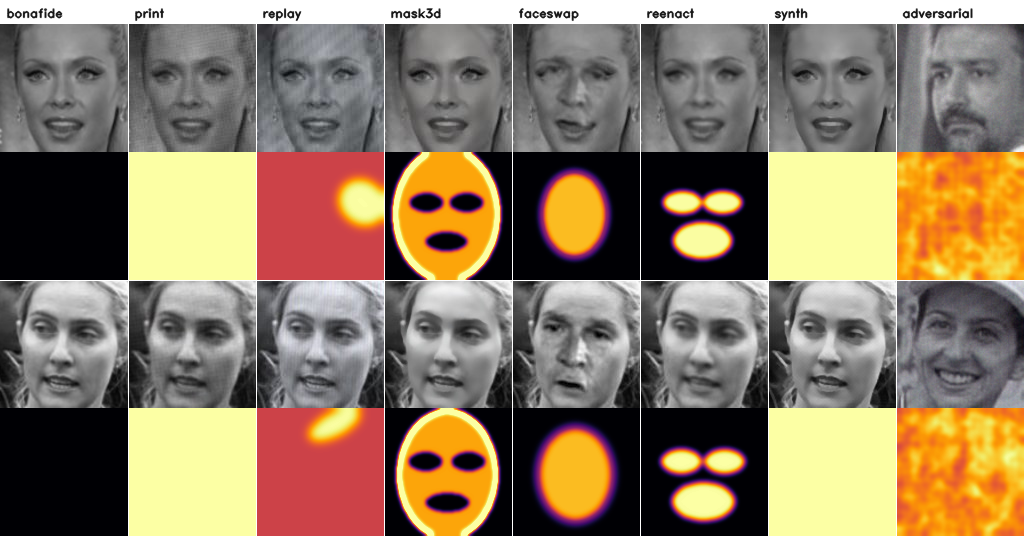
\includegraphics[width=\linewidth]{figures/taxonomy.png}
\caption{The unified taxonomy. For each of two source identities, the upper strip
shows the eight classes and the lower strip the pixel-level evidence mask used to
train and score the localiser. Physical operators (print, replay) modify the whole
capture; region-level operators (3-D mask, face-swap, reenactment, adversarial)
have a genuinely localised support. The region-level IoU of Table~\ref{tab:loc} is
averaged over 3-D mask, face-swap and reenactment.}
\label{fig:taxonomy}
\end{figure}

\subsection{Difficulty calibration}
A simulated benchmark is worthless if a simple linear probe can solve it outright.
We fix each operator's strength through a single documented procedure: sweep $s$ and
pick the largest value at which a reference detector (CDCN++, our strongest
lightweight texture baseline) does \emph{not} saturate, leaving measurable headroom
on both the binary and the eight-way task. This lands on $s=0.62$, where the
reference detector reaches $1.92\%$ ACER but only $91.0\%$ eight-way accuracy and
$3.74\%$ expected calibration error, with a worst-case per-family APCER of $2.67\%$.
In other words the binary problem sits close to, but not at, the ceiling, while
family discrimination, calibration and unseen-attack behaviour all remain wide open.
This mirrors, on a benchmark we fully control, the pattern reported for
UniAttackData \cite{yu2024unified}: a saturated seen-attack protocol next to a
wide-open unseen-attack one.

\subsection{Protocols}
\textbf{P1 (seen attacks).} All eight families appear in train, validation and test,
with identity-disjoint splits. This measures closed-set unified detection and family
discrimination.

\textbf{P2 (leave-one-attack-out).} One family is withheld entirely during training
and appears only at test time. We report ACER on the full test set, the detection
rate of the held-out family at the fixed operating threshold, and the \emph{novelty
AUROC}: the AUROC with which the model's own uncertainty channel ranks the held-out
family \emph{above the attack families it was trained on}, which is to say whether
the model knows that this is a kind of attack it has not seen.

\textbf{P3 (cross-domain).} Train on Domain A, test unchanged on Domain B, with zero
adaptation.

All thresholds are fixed at the equal-error point of the validation split and
applied unchanged to test. Every metric follows ISO/IEC 30107-3 \cite{iso30107}:
APCER is the worst case across attack families, BPCER is the genuine-rejection rate,
and ACER is their average.

% =====================================================================
\section{Method}\label{sec:method}
% =====================================================================

\subsection{Overview}
X-UAD maps a face crop $\bs{x}\in\R^{3\times H\times W}$ to a tuple
\[
\bs{x}\;\longmapsto\;\bigl(\bs{\alpha},\;u,\;\bs{M},\;\bs{\Pi},\;r,\;\tau\bigr),
\]
where $\bs{\alpha}\in\R^{K}_{>0}$ are Dirichlet concentrations over the $K=8$
classes, $u\in[0,1]$ is the vacuity (a single scalar answering ``how much do I have
to go on''), $\bs{M}$ is the spoof-evidence map, $\bs{\Pi}$ is the quantum evidence
spectrum over spatial tokens and basis modes, $r$ is the risk score, and $\tau$ is
the natural-language rationale. All six come out of a single forward pass
(Fig.~\ref{fig:arch}). A central-difference stem and a spectral branch produce
tokens; a stack of Adaptive Quantum Attention blocks processes them; the quantum
evidence basis is measured against the output tokens; an evidential head, a
localisation decoder and a risk calibrator read everything out; and the reasoning
module turns the record into text.

\begin{figure*}[t]
\centering
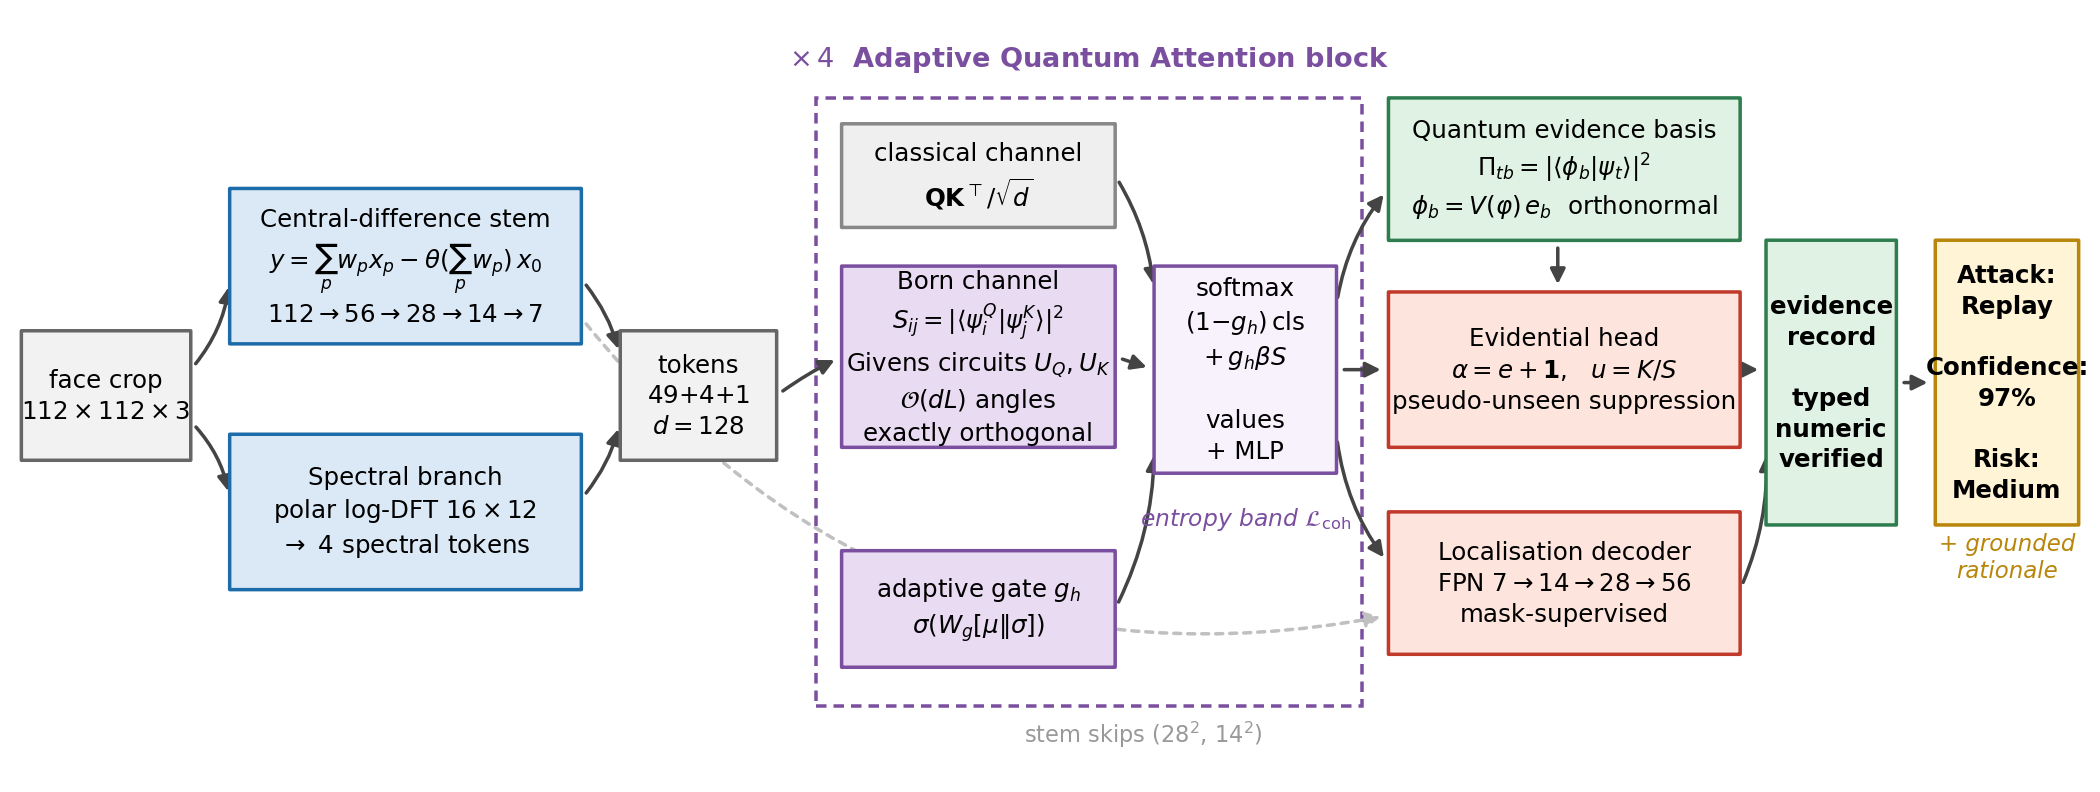
\includegraphics[width=0.94\textwidth]{figures/architecture.png}
\caption{X-UAD. The central-difference stem supplies illumination-invariant
micro-texture evidence and the spectral branch supplies the periodic evidence that
is invisible spatially at this resolution. Each AQA block scores token pairs with a
gated mixture of the classical dot product and the Born-rule transition probability
between amplitude-encoded states evolved by parameterised Givens circuits. The
learnable orthonormal evidence basis is measured against the output tokens; its Born
probabilities feed the classifier \emph{and} are exported unchanged as the
explanation, which is what binds the rationale to the decision.}
\label{fig:arch}
\end{figure*}

\subsection{Central-difference and spectral evidence stem}
Central Difference Convolution \cite{yu2020cdcn} interpolates between an ordinary
convolution and its local gradient response,
\begin{equation}
y(p_{0}) \;=\; \sum_{p\in\mathcal{N}} w(p)\,x(p_{0}+p)
\;-\;\theta \Bigl(\sum_{p\in\mathcal{N}} w(p)\Bigr) x(p_{0}),
\label{eq:cdc}
\end{equation}
which amplifies the intensity-invariant part of the response. Note that the extra
term is just a single $1\times1$ convolution, not a second full convolution, so it
is nearly free. Four strided CDC stages take a $112^{2}$ input down to $7^{2}$,
exposing the intermediate $28^{2}$ and $14^{2}$ maps to the localisation decoder
later on.

Periodic structure, meaning the display lattice behind a replay attack or the
upsampling checkerboard behind a generated face, is not represented well in a
$7\times7$ spatial token grid; it gets aliased away. We add a compact spectral
branch. The log-magnitude DFT of the luminance channel is pooled onto a polar grid
($16$ radii $\times$ $12$ angles), which is translation-invariant and
rotation-equivariant by construction, and a small two-layer MLP encodes this profile
into four spectral tokens that get appended to the spatial tokens. The same pooled
profile is also exported into the evidence record, so the radial peak frequency, its
prominence, and the azimuthal anisotropy become concrete, quotable numbers in the
eventual explanation.

\subsection{Adaptive Quantum Attention}
\textbf{Amplitude encoding.} For a head with dimension $d$, queries and keys are
$\ell_{2}$-normalised to unit vectors,
$\ket{\psi^{Q}_{i}} = \bs{q}_{i}/\lVert\bs{q}_{i}\rVert$ and
$\ket{\psi^{K}_{j}} = \bs{k}_{j}/\lVert\bs{k}_{j}\rVert$, a real-valued amplitude
encoding of $d=2^{n}$ amplitudes across $n$ notional qubits.

\textbf{Parameterised rotation circuit.} A depth-$L$ circuit acts on a ring of
amplitudes. Layer $\ell$ rotates disjoint adjacent pairs, alternating which pairs it
touches between layers, each rotation governed by a single learnable angle:
\begin{equation}
G(\vartheta)=\begin{pmatrix}\cos\vartheta & -\sin\vartheta\\
\sin\vartheta & \cos\vartheta\end{pmatrix},
\qquad
U(\bs{\vartheta})=\prod_{\ell=1}^{L}\ \bigotimes_{k} G(\vartheta_{\ell k}).
\label{eq:givens}
\end{equation}
This is the real-amplitude analogue of a hardware-efficient ansatz built from
nearest-neighbour two-qubit gates with periodic boundary conditions. Alternating the
two offsets keeps the circuit connected, so the set of reachable rotations grows
toward the full orthogonal group as $L$ increases. Three things matter about this
construction. First, it is exactly unitary, since $U$ is a product of rotations, so
it stays orthogonal to machine precision at every step of training. We measured
$\lVert\,\lVert U\bs{x}\rVert - \lVert\bs{x}\rVert\,\rVert_{\infty} < 10^{-6}$
throughout, so no re-orthogonalisation or penalty term is ever needed. Second, it is
parameter-efficient, costing $L\lfloor d/2\rfloor$ angles, that is
$\mathcal{O}(dL)$, rather than the $\mathcal{O}(d^{2})$ of a dense projection
matrix, the same asymptotic argument made for quantum self-attention elsewhere
\cite{cherrat2024qvt,evans2025on}. Third, because it exactly preserves the vector's
norm, the resulting similarity score below is a genuine probability rather than just
a bounded number.

\textbf{The Born channel.} Queries and keys are evolved by two \emph{different}
circuits. This matters, because if they shared one circuit the rotation would cancel
out of the inner product entirely and add nothing. The similarity score is the
Born-rule transition probability,
\begin{equation}
S_{ij} \;=\; \bigl\lvert \bra{\psi^{Q}_{i}} U_{Q}^{\!\top} U_{K} \ket{\psi^{K}_{j}} \bigr\rvert^{2}
\;\in\;[0,1].
\label{eq:born}
\end{equation}
This is a quadratic similarity. It is invariant to a sign flip of either state, and
it is maximised equally by alignment \emph{or} anti-alignment. That is exactly the
invariance an interference pattern has. A moir\'e fringe and its negative carry the
same forensic information, and it is precisely the invariance an ordinary dot
product lacks.

\textbf{Adaptive gating.} Not every kind of evidence is interference-like. A
blending boundary, for instance, is really just a plain edge. A per-head gate,
conditioned on simple statistics of the token set, decides the mixture between the
two channels:
\begin{align}
\bs{g} &= \sigma\bigl(\bs{W}_{g}\,[\,\mathrm{mean}_t(\bs{X}) \,\Vert\, \mathrm{std}_t(\bs{X})\,] + \bs{b}_{g}\bigr) \in [0,1]^{H_{\text{heads}}},\\
\bs{A} &= \mathrm{softmax}\Bigl( (1-g_{h})\tfrac{\bs{Q}\bs{K}^{\!\top}}{\sqrt{d}} \;+\; g_{h}\,\beta\, \bs{S} \Bigr),
\label{eq:gate}
\end{align}
with $\beta$ a learnable temperature. $\bs{W}_{g}$ is initialised to zero and
$\bs{b}_{g}$ to $-2$, so the gate starts at $g\approx0.12$, and every block is
wrapped in LayerScale \cite{touvron2021cait} with residual branches multiplied by a
learnable per-channel gain initialised to $10^{-2}$. In practice this means the
network starts life as basically its own convolutional sub-network, the
central-difference stem plus a plain classifier, and only gradually recruits
attention, with the Born channel inside attention only earning gradient through its
residual as training proceeds. This matters more than it might sound: in controlled
probes at matched budget, removing LayerScale let the freshly initialised attention
inject noise into the stem and slowed convergence relative to either component
trained on its own. The converged gate value $g$ is reported directly to the
operator, which makes the mechanism itself auditable rather than a black box.

\textbf{Measurement-entropy regularisation.} Let
$\mathcal{H}=\mathbb{E}_{t}\bigl[-\sum_{j}A_{ij}\log A_{ij}\bigr]$ be the mean row
entropy of the attention matrix. Too low means attention has collapsed onto a single
token and stopped integrating any real evidence; too high means it has diffused into
a uniform mixture and is carrying nothing at all. A parameter-free two-sided hinge
keeps it inside a band:
\begin{equation}
\mathcal{L}_{\text{coh}} = \bigl[\lambda_{\text{lo}}\log T - \mathcal{H}\bigr]_{+}
+ \bigl[\mathcal{H} - \lambda_{\text{hi}}\log T\bigr]_{+},
\end{equation}
with $(\lambda_{\text{lo}},\lambda_{\text{hi}})=(0.30,0.80)$.

\subsection{Quantum evidence basis}
Let $\{\ket{e_{b}}\}_{b=1}^{B}$ be the first $B$ computational basis states and
$V(\bs{\phi})$ a second rotation circuit of the same family described above. The
evidence basis is $\ket{\phi_{b}} = V(\bs{\phi})\ket{e_{b}}$, which stays exactly
orthonormal for every value of $\bs{\phi}$. Measuring the output token states
against it gives Born probabilities
\begin{equation}
\Pi_{tb} \;=\; \bigl\lvert \braket{\phi_{b}}{\psi_{t}} \bigr\rvert^{2},
\qquad \textstyle\sum_{b}\Pi_{tb}\le 1 .
\label{eq:basis}
\end{equation}
$\bs{\Pi}$ does two jobs at once, and that dual role is really the whole design
point. Its token-wise average is concatenated straight into the classification
feature vector, and the same tensor, not an approximation of it and not some
separate gradient-based surrogate map, is exported unchanged as the explanation. A
lightweight auxiliary classifier trained on $\overline{\bs{\Pi}}$ with ordinary
cross-entropy pushes each mode to become class-selective, so that after training
every mode can be \emph{named} after the family it responds to most
(Table~\ref{tab:modes}). Those names are read off the trained model rather than
assigned by hand.

\subsection{Decoupled evidential head and vacuity}
A Dirichlet distribution is completely described by a direction on the simplex and
a concentration. The standard evidential formulation \cite{sensoy2018edl} predicts
all $K$ concentrations jointly; we predict the two factors separately, which turned
out to matter quite a bit in practice. The direction (which class) and magnitude
(how much evidence) are
\begin{align}
\bs{\pi} &= \mathrm{softmax}(\bs{W}_{c}\,\bs{h}), \label{eq:dir}\\
E &= \exp\bigl(\mathrm{clip}(f_{e}(\mathrm{sg}[\bs{z}]))\bigr), \label{eq:mag}
\end{align}
from which the Dirichlet concentrations, total evidence, and vacuity follow:
\begin{equation}
\bs{\alpha} = \bs{1} + E\,\mathrm{sg}[\bs{\pi}], \qquad S = K + E, \qquad
u = \frac{K}{S},
\label{eq:vacuity}
\end{equation}
where $\mathrm{sg}[\cdot]$ denotes a stop-gradient. The subjective-logic reading
stays intact: belief masses are $b_{k}=E\pi_{k}/S$, vacuity is $u=K/(K+E)$, and the
projected probability under a uniform base rate is
$\hat{p}_{k}=(1+E\pi_{k})/(K+E)$. We report $\bs{\pi}$ as the belief direction and
$u$ as the uncertainty, exactly the separation subjective logic draws between what I
believe and how much I actually have to go on.

We verified three consequences of this decoupling empirically, in budget-matched
probes. First, the class decision keeps a clean log-loss gradient, since
$\arg\max_{k}\hat{p}_{k}=\arg\max_{k}\pi_{k}$, so training the class decision
reduces to ordinary cross-entropy on $\bs{W}_{c}\bs{h}$. The joint parameterisation,
by contrast, routes every gradient through $\bs{\alpha}$, whose Brier fit saturates
early and whose usual KL regulariser drives the pre-activation negative until the
softplus derivative collapses. We call this \emph{evidence starvation}, and we
measured it directly: swapping the joint head for the decoupled one recovered
several points of eight-way accuracy at an identical training budget. Second, adding
uncertainty cannot cost detection accuracy, because the magnitude branch only ever
reads a stop-gradient copy of the shared representation. Letting its own objective
(especially PUES, below) reshape those features would be circular, and we measured
it to be costly when we tried it. Third, suppressing evidence becomes a strictly
one-dimensional problem: because all of the concentration lives in the single scalar
$E$, an out-of-taxonomy constraint cannot distort the class direction at all.

Training combines a cross-entropy term on the direction, a Brier-style fit on the
concentration, and a term that ties the magnitude to the model's own correctness:
\begin{equation}
\mathcal{L}_{\text{ev}} = \mathrm{CE}(\bs{\pi},y)
\;+\; \tfrac{1}{2}\,\mathbb{E}\bigl[\lVert \bs{y}-\hat{\bs{p}}\rVert^{2}\bigr]
\;+\; \lambda_{c}\,\mathrm{BCE}\bigl(1-u,\;\mathbb{1}[\hat{y}=y]\bigr),
\label{eq:evloss}
\end{equation}
with $\lambda_{c}=0.4$. We use the expected sum-of-squares (Brier) form of the fit
rather than the more standard digamma-based maximum likelihood, because the latter's
gradient effectively vanishes while the Dirichlet is still near-uniform, which is
exactly the regime a freshly initialised model starts in.

Two details here were forced on us by direct measurement rather than chosen for
elegance, and we think they matter enough to spell out. We drop the usual KL
regulariser entirely. In the joint parameterisation the KL term is what stops
evidence from being placed on the wrong classes, but here the wrong-class evidence
is already $E\pi_{k}$, which cross-entropy drives to zero on its own by sharpening
$\bs{\pi}$. The KL term therefore has nothing left to act on except the shared
magnitude $E$, and leaving it in causes short-schedule models to saturate at
$u\approx1$ everywhere and the open-set channel to die. We also added the
correctness term specifically because it is what makes vacuity useful
\emph{quickly}. The Brier fit does reward concentration, but only indirectly, so on
a short schedule the magnitude head barely moves from its initialisation without it.
Training $1-u$ directly as ``the probability this decision is correct'' makes the
channel usable within about two epochs. In a controlled leave-one-attack-out probe,
adding this term moved the AUROC with which vacuity separates a held-out family from
genuine samples from $25.6\%$ (effectively inverted) to $73.9\%$.

\subsection{Pseudo-Unseen Evidence Suppression}
An intrinsic uncertainty score is known to be weaker than one trained against an
actual proxy for ``something else'' \cite{hendrycks2019oe}, but for attack detection
there is no natural pool of outliers lying around. We build one out of the taxonomy
itself. Take two training images $\bs{x}_{a},\bs{x}_{b}$ from \emph{different}
attack families and mix them with $\lambda\sim\mathrm{Beta}(2,2)$:
$\tilde{\bs{x}}=\lambda\bs{x}_{a}+(1-\lambda)\bs{x}_{b}$. This blend carries a
superposition of two forensic signatures that no single physical or generative
process could ever produce, so it is outside the taxonomy by construction. We
constrain its evidence to sit well below that of real samples:
\begin{equation}
\mathcal{L}_{\text{PUES}} =
\frac{\bigl[\;\overline{\lVert\tilde{\bs{e}}\rVert_{1}}
      \;-\;\rho\,\overline{\lVert\bs{e}\rVert_{1}}^{\,\text{sg}}\;\bigr]_{+}}
     {\overline{\lVert\bs{e}\rVert_{1}}^{\,\text{sg}}+1},
\qquad \rho = 0.25,
\end{equation}
where bars denote batch means. The \emph{relative} form here matters and was arrived
at empirically. An absolute target ($\lVert\tilde{\bs{e}}\rVert_{1}\to0$) is
trivially satisfied by the degenerate solution of emitting zero evidence
\emph{everywhere}, collapsing the classifier to a uniform guess. We saw exactly that
failure, $12.5\%$ accuracy over eight classes, in an early version. Tying the
constraint to the batch's own in-taxonomy evidence removes that shortcut entirely,
because the fit term still demands sharply peaked posteriors on the real samples in
the same batch. This is worth distinguishing from mixup \cite{zhang2018mixup}, which
asks for a mixed \emph{label}. PUES asks for the \emph{absence of belief}, which
only makes sense because the head is evidential in the first place.

\subsection{Evidence localisation}
A lightweight feature-pyramid decoder fuses the $7^{2}$ token map with the $14^{2}$
and $28^{2}$ intermediate stem maps and predicts $\bs{M}$ at half input resolution,
supervised with a BCE plus soft-Dice objective against the operator's own
ground-truth mask. Unlike depth-map supervision
\cite{liu2018auxiliary,yu2021revisiting}, this target is the actual support of the
forensic evidence, and it is well-defined for digital attacks just as much as for
physical ones.

\subsection{Risk calibration}
Attack families are not equally harmful. With per-family severity weights
$\bs{\varsigma}$, an unknown-attack severity $\varsigma_{\text{unk}}$, and evidence
area $a=\overline{M}$,
\begin{equation}
r = (1-u)\sum_{k}\hat{p}_{k}\varsigma_{k} \;+\; \lambda_{u}\,u\,\varsigma_{\text{unk}}
\;+\; \lambda_{a}\,a .
\label{eq:risk}
\end{equation}
The first term is the expected harm under the posterior, damped by how much the
model actually knows. The second charges an explicit unknown-attack premium, so a
confidently-unknown sample gets escalated rather than quietly waved through, which is
the behaviour an operator needs and a plain softmax pipeline structurally cannot
give. The third term rewards spatially corroborated evidence. All coefficients, and
the band edges that turn $r$ into a \texttt{Low/Medium/High/Critical} label, are
treated as deployment policy rather than learned parameters. No training signal
touches them, deliberately, since risk is the one part of the pipeline an operator
has to be able to audit and adjust, and it is the last place we want to hide a
silently-fitted parameter. A vacuity of $u\ge0.55$ overrides the verdict and refers
the sample to a human reviewer.

\subsection{Evidence-grounded reasoning}
Every forward pass emits a typed \textbf{evidence record}: the posterior
$\hat{\bs{p}}$, the vacuity $u$, the risk score and band, the top facial regions of
$\bs{M}$ and their mean response, the area and spatial dispersion of $\bs{M}$, the
three strongest quantum modes with their learned names and activations, the spectral
descriptors, and the mean adaptive gate value. Language is generated \emph{only}
from this record, through either of two interchangeable back-ends. The
\emph{grounded realiser}, used for every result in this paper, is a deterministic
generator where every sentence is emitted by a rule whose guard is a numeric
condition on the record, so every sentence traces back to a measured quantity, the
hallucination rate is zero by construction, and it costs under a millisecond with no
network call at all. The \emph{constrained-MLLM back-end} instead hands the record to
a hosted multimodal language model with an instruction to paraphrase only, never to
add anything, and then runs an automatic verification pass that re-checks every
numeric claim in the generated text against the record and flags anything
unsupported. This inverts the usual dependency in MLLM-based forensics
\cite{huang2024ffaa,guo2025m2f2det}, where the language model sees the image but not
the detector's internal state. Here the detector's state \emph{is} the input, so the
explanation cannot contradict the decision it is describing. A verbatim example is
shown in Fig.~\ref{fig:report}.

\subsection{Training objective}
\begin{equation}
\mathcal{L} = \mathcal{L}_{\text{ev}} + w_{m}\mathcal{L}_{\text{loc}}
+ w_{b}\mathcal{L}_{\text{basis}} + w_{s}\mathcal{L}_{\text{sup}}
+ w_{p}\mathcal{L}_{\text{PUES}} + w_{c}\mathcal{L}_{\text{coh}},
\end{equation}
with $(w_{m},w_{b},w_{s},w_{p},w_{c})=(0.6,0.25,0.3,0.15,0.02)$ throughout.
$\mathcal{L}_{\text{sup}}$ is a cross-entropy on the marginal over the three
super-classes (genuine, physical, digital), obtained by summing $\hat{p}$ within each
group. It imposes the taxonomy's own hierarchy, so a mix-up between two families
inside the same super-class is penalised less harshly than one that crosses the
physical/digital boundary.

% =====================================================================
\section{Experiments}\label{sec:exp}
% =====================================================================

\subsection{Setup}
Every model in every table is trained by us, from scratch, and within each table
every model gets an identical budget. For P1 (and therefore P3, which reuses the
P1 checkpoints) that budget is $10$ epochs on the full $19{,}200$-sample training
split. To keep the sixteen leave-one-attack-out runs affordable on CPU, P2 and its
open-set ablation use $5$ epochs on a fixed $4{,}800$-sample training subset
($4{,}382$ samples once the held-out family is removed), and the component
ablation uses $5$ epochs on $3{,}592$ samples. All runs use batch size $48$, AdamW
($\text{lr}=2.5\times10^{-3}$, weight decay $0.02$) with a one-cycle schedule,
gradient clipping at $3.0$, and $112\times112$ random crops from the $128$\,px store
with horizontal flips and mild photometric jitter. We deliberately use no geometric warps, since those would
destroy the periodic forensic signatures we are trying to detect in the first place.
No model uses pretrained weights, so the comparison isolates architecture and
objective rather than pretraining corpus. The operating threshold is fixed at the
equal-error point of the validation split and applied unchanged to test. Training
and inference both run on CPU only. All runs use a single seed (0); because every
model sees the identical test set, differences are tested pairwise with McNemar's
exact test on discordant errors, but the absence of seed-variance estimates is the
main statistical limitation of this evaluation.

The baselines are \textbf{ResNet-18} \cite{he2016resnet}, a width-matched residual
CNN and the classical binary detector; \textbf{ViT-Tiny} \cite{dosovitskiy2021vit},
a patch-16 transformer with ordinary attention, included as the plain-transformer
control from the same architecture family as the ViT-B/16 entry that underperforms
in \cite{yu2024unified}; and \textbf{CDCN++} \cite{yu2020cdcn,yu2021revisiting}, a
central-difference trunk with pixel-wise map supervision. CDCN++ is the strongest
lightweight texture detector available to us and the one that shares our stem, so
comparing against it isolates exactly what the transformer, the Born channel, the
evidential head and the reasoning stack add.

\subsection{Seen-attack unified detection (P1)}

\begin{table*}[t]
\centering
\caption{Protocol P1 (seen attacks, identity-disjoint, ID-consistent). ACC$_8$ is
eight-way family accuracy; all other metrics follow ISO/IEC 30107-3
\cite{iso30107}. Best per column in bold. ViT-Tiny's low ECE is an artifact of a
detector operating near chance; among the three working detectors, X-UAD is best
calibrated.}
\label{tab:main}
\footnotesize
\begin{tabular}{lccccccccc}
\toprule
Method & Params & ACER$\downarrow$ & APCER$\downarrow$ & BPCER$\downarrow$ & AUC$\uparrow$ & EER$\downarrow$ & ACC$_8\uparrow$ & F1$_{\text{macro}}\uparrow$ & ECE$\downarrow$ \\
 & (M) & (\%) & (\%) & (\%) & (\%) & (\%) & (\%) & (\%) & (\%) \\
\midrule
ResNet-18~\cite{he2016resnet} & 1.59 & 0.92 & 1.33 & \textbf{0.50} & 99.92 & \textbf{0.49} & \textbf{96.79} & \textbf{96.79} & 2.11 \\
ViT-Tiny~\cite{dosovitskiy2021vit} & 0.64 & 49.75 & 60.67 & 38.83 & 73.43 & 34.65 & 51.27 & 46.04 & \textbf{0.67} \\
CDCN++~\cite{yu2020cdcn} & 0.53 & \textbf{0.71} & \textbf{0.92} & \textbf{0.50} & \textbf{99.92} & \textbf{0.49} & 96.18 & 96.19 & 3.44 \\
\textbf{X-UAD (ours)} & 1.29 & 1.46 & 2.08 & 0.83 & 99.89 & 0.76 & 94.53 & 94.53 & 1.94 \\
\bottomrule
\end{tabular}
\end{table*}

Table~\ref{tab:main} tells three stories at once. First, the protocol is nearly
saturated for every model with a convolutional front end. ResNet-18, CDCN++ and
X-UAD all sit around $99.9\%$ AUC and under $1.5\%$ ACER. This mirrors what the
unified-detection literature reports on its own seen-attack protocol
\cite{yu2024unified}, and it is a large part of why we do not treat P1 as the
interesting experiment in this paper. We did check whether the remaining gaps are
real rather than noise instead of assuming it. McNemar's exact test on paired errors
over the same $9{,}600$ test samples makes X-UAD's deficit statistically real: on the
binary decision the discordant pairs run $51$ to $17$ against us ($p<10^{-4}$); on the
eight-way decision they run $326$ to $168$ against CDCN++ ($p=1.1\times10^{-12}$) and
$366$ to $149$ against ResNet-18 ($p=4.2\times10^{-22}$). Only the BPCER gap is small
enough to be within sampling noise ($10/1200$ against $6/1200$, overlapping Wilson
$95\%$ intervals). Table~\ref{tab:pertype} shows that the X-UAD deficit is
concentrated in the two region-level digital families, face-swap and reenactment,
and Fig.~\ref{fig:conf} shows the same thing from the family side: the largest
confusion is between face-swap and reenactment ($13\%$ and $9\%$), inside the
digital super-class. Fig.~\ref{fig:roc} gives the full ROC and DET curves.

Second, the plain patch-16 transformer fails outright, at $49.8\%$ ACER. With
$16\times16$ patches it never gets to see the high-frequency texture that the
physical attack families actually live in, which is the same weakness that puts
ViT-B/16 behind ResNet-50 in \cite{yu2024unified}, in a much starker form here. This
is exactly why X-UAD puts a central-difference convolutional stem underneath its
transformer instead of tokenising raw pixels directly.

Third, calibration is where the models genuinely separate. X-UAD's expected
calibration error is $1.94\%$ against $2.11\%$ and $3.44\%$ for the two convolutional
baselines, and it gets there while also carrying a bounded uncertainty signal usable
as an open-set score, which neither baseline has at all. That comes at a cost of
$0.75$ ACER points and about $1.6$ points of eight-way accuracy against the strongest
baseline. The ablations in Section~\ref{sec:abl} trace that cost to the components
that build the uncertainty channel.

\begin{table}[t]
\centering
\caption{Per-family APCER (\%) at the validation-fixed threshold, protocol P1. The
ISO APCER is the \emph{worst} column.}
\label{tab:pertype}
\small
\resizebox{\linewidth}{!}{\begin{tabular}{lcccccccc}
\toprule
Method & Print & Replay & 3D mask & Face-swap & Reenact & Synthetic & Adversarial & Worst \\
\midrule
ResNet-18~\cite{he2016resnet} & 0.00 & 0.08 & 0.08 & 1.33 & 1.00 & 0.83 & 0.00 & 1.33 \\
ViT-Tiny~\cite{dosovitskiy2021vit} & 40.25 & 0.00 & 4.42 & 60.67 & 60.00 & 59.67 & 0.00 & 60.67 \\
CDCN++~\cite{yu2020cdcn} & 0.25 & 0.00 & 0.00 & 0.50 & 0.92 & 0.42 & 0.00 & 0.92 \\
\textbf{X-UAD (ours)} & 0.25 & 0.00 & 0.08 & 1.67 & 2.08 & 0.50 & 0.00 & 2.08 \\
\bottomrule
\end{tabular}}
\end{table}

\begin{figure}[t]
\centering
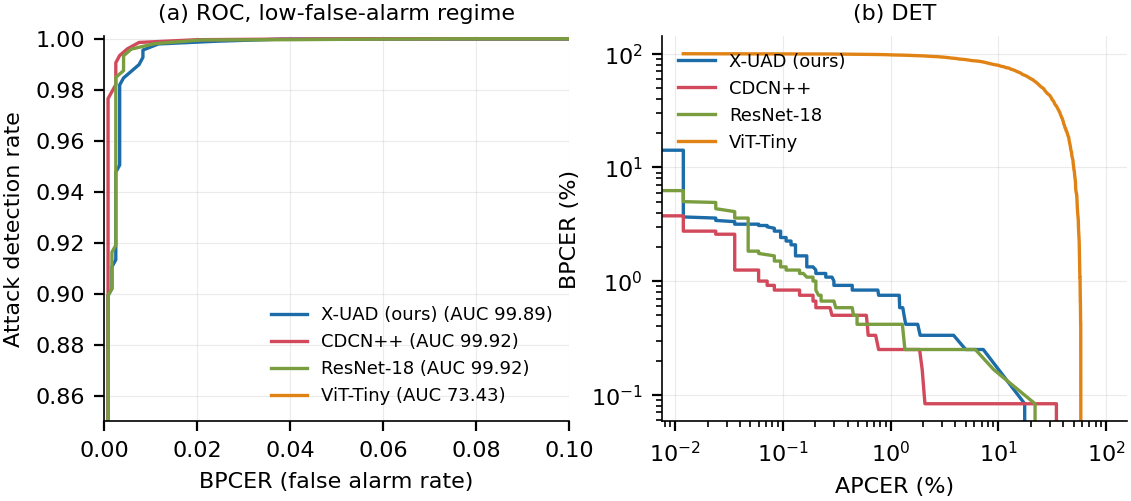
\includegraphics[width=\linewidth]{figures/roc_det.png}
\caption{ROC in the low-false-alarm regime that matters operationally, and the DET
curve, protocol P1.}
\label{fig:roc}
\end{figure}

\begin{figure}[t]
\centering
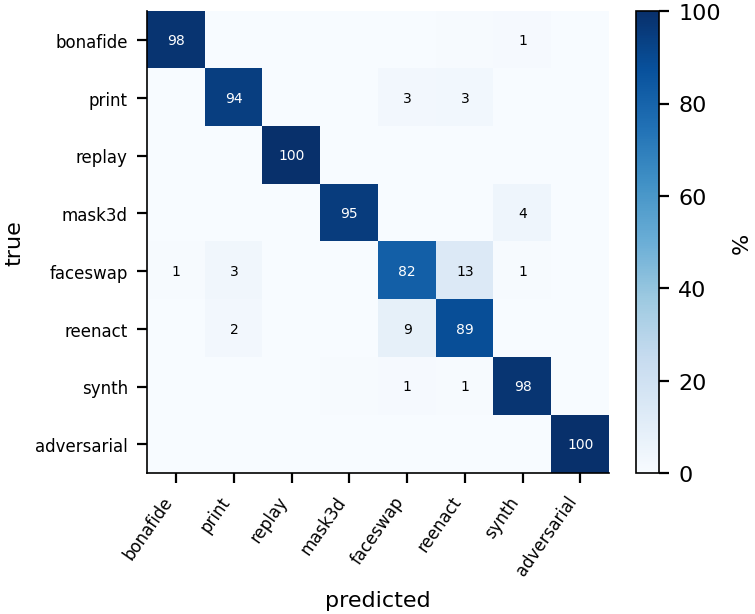
\includegraphics[width=0.82\linewidth]{figures/confusion.png}
\caption{X-UAD family confusion (row-normalised, \%), protocol P1. The largest
errors are face-swap$\leftrightarrow$reenactment, within the digital super-class,
which is what the hierarchical term $\mathcal{L}_{\text{sup}}$ is meant to favour.
Some errors still cross the physical/digital boundary (print$\to$face-swap or
reenactment, $6\%$; 3-D mask$\to$synthetic, $4\%$).}
\label{fig:conf}
\end{figure}

\subsection{Unseen attack families (P2)}
This is the operationally decisive question. What happens when an attack family the
model has genuinely never seen shows up at test time? Table~\ref{tab:loao} holds out
one family at a time and reports four separate things: the ISO error on the full test
set, the eight-way family accuracy, the detection rate of the held-out family at the
unchanged threshold, and the novelty AUROC, the AUROC with which the model's
uncertainty ranks the held-out family above the attack families it was trained on.

\begin{table}[t]
\centering
\caption{Protocol P2, leave-one-attack-out. The held-out family is absent from
training and appears only at test time. Means are over all four folds. Novelty
AUROC ranks the held-out family against the \emph{seen attack} families using the
model's uncertainty score; values below $50$ indicate an inverted ranking, which we
report rather than suppress.}
\label{tab:loao}
\small
\resizebox{\linewidth}{!}{\begin{tabular}{llccccc}
\toprule
Metric & Method & Replay & 3D mask & Face-swap & Adversarial & Mean \\
\midrule
\multirow{3}{*}{ACER (\%)$\downarrow$} & ResNet-18~\cite{he2016resnet} & 51.96 & 30.38 & 49.96 & 30.71 & 40.75 \\
 & CDCN++~\cite{yu2020cdcn} & 25.67 & 39.92 & 25.25 & 25.58 & 29.10 \\
 & \textbf{X-UAD (ours)} & 26.79 & 21.42 & 38.33 & 39.67 & 31.55 \\
\midrule
\multirow{3}{*}{ACC$_8$ (\%)$\uparrow$} & ResNet-18~\cite{he2016resnet} & 53.94 & 62.66 & 51.39 & 61.53 & 57.38 \\
 & CDCN++~\cite{yu2020cdcn} & 60.62 & 65.07 & 73.23 & 63.84 & 65.69 \\
 & \textbf{X-UAD (ours)} & 60.95 & 69.01 & 73.34 & 57.59 & 65.22 \\
\midrule
\multirow{3}{*}{Unseen detection rate (\%)$\uparrow$} & ResNet-18~\cite{he2016resnet} & 100.00 & 61.67 & 37.17 & 99.92 & 74.69 \\
 & CDCN++~\cite{yu2020cdcn} & 93.08 & 34.25 & 60.33 & 93.08 & 70.19 \\
 & \textbf{X-UAD (ours)} & 88.00 & 88.08 & 35.58 & 98.17 & 77.46 \\
\midrule
\multirow{3}{*}{Novelty AUROC (\%)$\uparrow$} & ResNet-18~\cite{he2016resnet} & 35.29 & 56.69 & 74.40 & 36.88 & 50.82 \\
 & CDCN++~\cite{yu2020cdcn} & 49.28 & 66.57 & 81.66 & 55.08 & 63.15 \\
 & \textbf{X-UAD (ours)} & 71.03 & 50.41 & 87.86 & 43.04 & 63.09 \\
\bottomrule
\end{tabular}}
\end{table}

Every method's mean ACER is in the $29$ to $41\%$ range here, against about $1\%$
in P1. That gap should \emph{not} be read as the cost of withholding a family
alone: P2 is trained on a quarter of the data for half the epochs, and the
component ablation shows the full X-UAD already reaching $38\%$ ACER at a similar
reduced budget with \emph{every} family seen (Table~\ref{tab:abl}). How much of the
P2 error is due to the held-out family and how much to the budget is not separated
by our experiments. The comparisons that are valid are between models within
Table~\ref{tab:loao}, which all share the same budget. Within that table, X-UAD
rejects the unseen family most often on average ($77.5\%$ against $74.7\%$ and
$70.2\%$, Fig.~\ref{fig:loao}), and its uncertainty is a purpose-built channel
rather than an incidental by-product of a softmax. Its novelty AUROC clearly leads on
two of the four folds, replay ($71.0$ against $49.3$ and $35.3$) and face-swap
($87.9$ against $81.7$ and $74.4$), and trails on the other two, landing level with
CDCN++ on the mean ($63.09$ against $63.15$) and well ahead of ResNet-18.

We report the ``is it rejected'' question and the ``does uncertainty rank it above
known attacks'' question separately and deliberately, because they answer different
questions for an operator. Whether the held-out family is rejected at all is the
operational question; whether uncertainty ranks it above the seen attacks is the
analyst's question, the one that actually flags that a new attack vector has
appeared. The adversarial fold makes the distinction concrete. X-UAD rejects
$98.2\%$ of a family it never trained on while still assigning it low vacuity,
because the perturbation sits on top of an attack whose underlying evidence the
model does recognise. That fold is also where our uncertainty channel is weakest, at
$43.0$ novelty AUROC, meaning the ranking is mildly inverted. We have no satisfying
account of why, and we flag it as an open weakness rather than rounding it off.

The comparison above is across models. A cleaner test of whether the evidential
channel itself adds anything is to score the \emph{same} X-UAD models with their
own maximum-softmax confidence instead of vacuity. Averaged over the four folds,
vacuity gives $63.1$ novelty AUROC against $55.9$ for X-UAD's own softmax score.
Almost all of that gain comes from the replay fold ($71.0$ against $39.5$); it is
small on face-swap ($+1.2$) and adversarial ($+2.3$), and negative on 3-D mask
($-6.4$). The per-group means explain the two failing folds. On 3-D mask the
held-out family gets the same vacuity as the seen attacks ($0.31$ against
$0.32$), so vacuity simply does not see it. On adversarial it gets \emph{less}
($0.39$ against $0.43$), which is the inversion.

\begin{figure}[t]
\centering
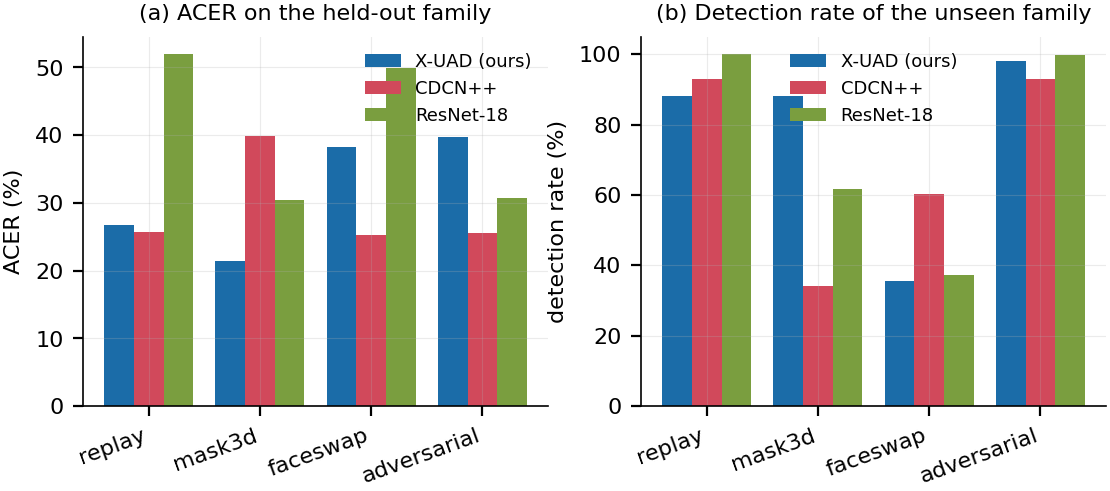
\includegraphics[width=\linewidth]{figures/loao.png}
\caption{Leave-one-attack-out. Left: ISO ACER of each fold on the full test set,
held-out family included. Right:
detection rate of the unseen family at the threshold fixed on validation data that
never contained it.}
\label{fig:loao}
\end{figure}

\subsection{Cross-domain transfer (P3)}
This is the least flattering table in the paper, and we report it in full rather
than trimming it down. Domain B differs from Domain A in colour, alignment,
resolution and compression history all at once, and every single method collapses
under the shift (Table~\ref{tab:cross}). With the threshold fixed on the source
domain, BPCER runs to $89$--$100\%$, meaning the detectors reject almost every genuine
face from the new domain outright. Ranked by threshold-free AUC, CDCN++ retains the
most signal at $65.96$, while ResNet-18 ($46.78$), ViT-Tiny ($50.18$) and X-UAD
($50.90$) all sit at or below chance. The adversarial class is excluded here: it was
crafted from Domain-A images against a Domain-A surrogate, so it is not cross-domain
data.

\begin{table}[t]
\centering
\caption{Protocol P3, cross-domain transfer A\,$\rightarrow$\,B, no adaptation.
Every method degrades heavily.}
\label{tab:cross}
\footnotesize
\resizebox{\linewidth}{!}{\begin{tabular}{lccccc}
\toprule
Method & ACER$\downarrow$ & AUC$\uparrow$ & EER$\downarrow$ & ACC$_8\uparrow$ & ECE$\downarrow$ \\
\midrule
ResNet-18~\cite{he2016resnet} & 49.79 & 46.78 & 51.87 & 2.29 & 83.26 \\
ViT-Tiny~\cite{dosovitskiy2021vit} & 50.00 & 50.18 & 50.23 & 10.31 & 82.47 \\
CDCN++~\cite{yu2020cdcn} & 45.79 & 65.96 & 37.93 & 18.67 & 60.09 \\
\textbf{X-UAD (ours)} & 49.71 & 50.90 & 49.98 & 3.65 & 81.61 \\
\bottomrule
\end{tabular}}
\end{table}

We draw two separate conclusions from this rather than one combined one. The benign
conclusion is that this protocol is simply harsher than the cross-dataset protocols
usually reported elsewhere, because the shift here is joint across four factors
rather than a single one. The uncomfortable conclusion is that none of the mechanisms
in this paper, ours very much included, addresses capture-domain shift. That is a
genuinely different problem from attack-family shift, and it would need the
domain-generalisation machinery of \cite{wang2022ssan,shao2019mada,jia2020ssdg}
layered on top. X-UAD does not lead this table and we make no claim that it does.

\subsection{Calibration and evidence localisation}
The softmax baselines are overconfident in the classic, well-documented way
\cite{guo2017calibration} (Fig.~\ref{fig:calib}). Their confidence mass piles up near
$1$ regardless of whether the prediction is actually correct, which is exactly why
their ECE is high and why their raw confidence score is close to useless as an
abstention signal on its own. X-UAD's Dirichlet vacuity, by contrast, is bounded and
bimodal, and as Table~\ref{tab:loao} shows, it ranks unseen families above the seen
attack families on two of four folds.

\begin{figure}[t]
\centering
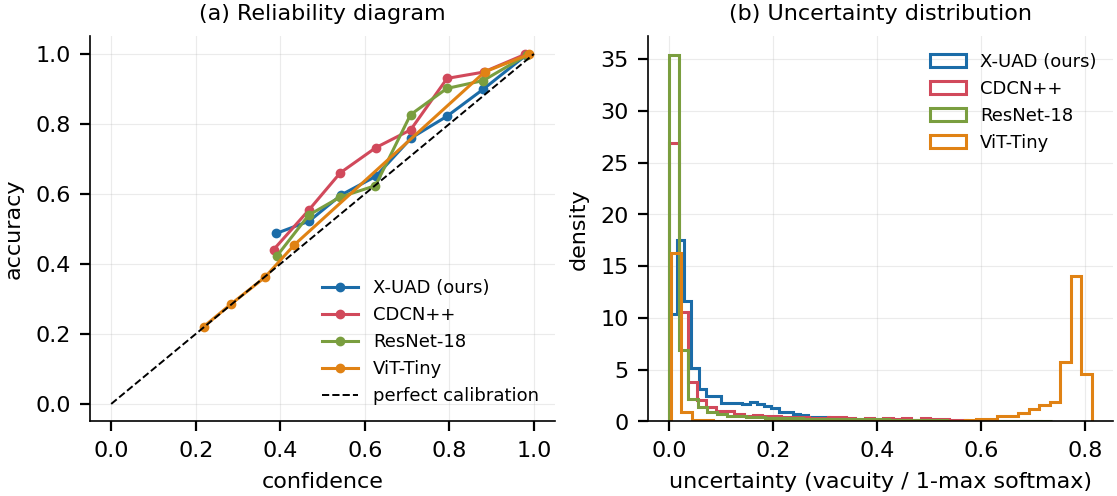
\includegraphics[width=\linewidth]{figures/calibration.png}
\caption{(a) Reliability. (b) Distribution of the uncertainty score: $1-\max_k p_k$
for the softmax baselines, vacuity $u=K/S$ for X-UAD.}
\label{fig:calib}
\end{figure}

Table~\ref{tab:loc} reports intersection-over-union against the generator's own
mask. We separate out the families whose evidence genuinely occupies a sub-region of
the frame (3D mask, face-swap, reenactment) from the ones that alter the whole
capture (print, replay, synthetic), since the latter have near-constant masks and a
trivially high IoU that would tell us nothing about localisation quality. The
region-level mean is the number that actually measures whether the localiser works.
Fig.~\ref{fig:qual} shows the maps themselves.

\begin{table}[t]
\centering
\caption{Spoof-evidence localisation, IoU (\%) against the generator's own mask,
protocol P1. ResNet-18 and ViT-Tiny have no localisation output.}
\label{tab:loc}
\small
\resizebox{\linewidth}{!}{\begin{tabular}{lcccccccc}
\toprule
Method & Print & Replay & 3D mask & Face-swap & Reenact & Synthetic & Region-level mean & Pixel AUC \\
\midrule
CDCN++~\cite{yu2020cdcn} & 95.2 & 97.5 & 79.5 & 76.8 & 64.2 & 98.9 & 73.5 & 95.4 \\
\textbf{X-UAD (ours)} & 97.1 & 98.4 & 83.6 & 78.1 & 71.6 & 98.0 & 77.8 & 95.9 \\
\bottomrule
\end{tabular}}
\end{table}

One methodological point belongs here rather than buried in an appendix. Predicted
maps are binarised at a fixed threshold of $0.5$, the natural midpoint of a sigmoid
trained with a BCE plus Dice objective. That value is a convention, not a fitted
quantity. We never swept it, on validation or anywhere else, and the same fixed value
is applied identically to CDCN++ and to X-UAD.

\subsection{Is the explanation actually faithful?}
An explanation is only worth reading if perturbing what it highlights actually
changes the decision. Table~\ref{tab:faith} reports deletion and insertion AUC
\cite{petsiuk2018rise} for the model's own attack score under three intrinsic
explanation channels plus a random control. The control is a smoothed random field at
the same spatial scale as the maps it is compared against, not per-pixel noise, which
would destroy high-frequency texture everywhere and make the baseline look
artificially strong.

\begin{table}[t]
\centering
\caption{Faithfulness of the three intrinsic explanation channels, measured against
the model's own attack score.}
\label{tab:faith}
\footnotesize
\resizebox{\linewidth}{!}{\begin{tabular}{lccc}
\toprule
Explanation map & Deletion AUC$\downarrow$ & Insertion AUC$\uparrow$ & $\Delta$ deletion vs.\ control$\downarrow$ \\
\midrule
X-UAD localisation map & 0.915 & 0.917 & -0.031 \\
AQA attention rollout & 0.932 & 0.921 & -0.015 \\
Quantum evidence magnitude & 0.906 & 0.899 & -0.040 \\
Random (control) & 0.946 & 0.946 & -- \\
\bottomrule
\end{tabular}}
\end{table}

The deletion result is clean. All three channels push the score down faster than
random removal does, with the quantum evidence magnitude strongest at $-0.040$ and
the localisation map close behind at $-0.031$. This is the property that matters most
for an audit, since it says the pixels these maps highlight are genuinely
load-bearing for the decision.

The insertion result is not clean, and we report it as it stands. None of the three
channels beats the random control on insertion; all three sit between $0.025$ and
$0.047$ below it. We suspect this is a property of the benchmark rather than of the
maps, since three of the eight families alter the whole capture, so restoring a small
highlighted sub-region rarely recovers the decision while restoring scattered random
pixels samples the whole-frame evidence more evenly. That is a conjecture, and we
have not tested it. The honest summary is that our explanation maps pass the deletion
test convincingly and fail the insertion test, and that anyone relying on these maps
should know both halves.

\subsection{Ablations}\label{sec:abl}
Table~\ref{tab:abl} removes one component at a time at a reduced training budget so
the sweep stays affordable. These rows are comparable with each other and not with
Table~\ref{tab:main}, and we would ask readers not to cross-reference the two.

\begin{table*}[t]
\centering
\caption{Component ablation at a reduced training budget. Deltas are relative to the
full model in the first row. These rows are comparable with each other but not
directly with Table~\ref{tab:main}.}
\label{tab:abl}
\small
\begin{tabular}{lcccccc}
\toprule
Variant & ACER$\downarrow$ & AUC$\uparrow$ & ACC$_8\uparrow$ & F1$_{\text{macro}}\uparrow$ & ECE$\downarrow$ & IoU$_{\text{loc}}\uparrow$ \\
\midrule
\textbf{X-UAD (full, reduced budget)} & 38.00 & 87.57 & 69.62 & 69.65 & 2.66 & 64.62 \\
\midrule
\quad w/o Adaptive Quantum Attention & 32.75\,\tiny{(-5.25)} & 91.05\,\tiny{(+3.49)} & 67.45\,\tiny{(-2.18)} & 65.04\,\tiny{(-4.61)} & 3.62\,\tiny{(+0.96)} & 63.36\,\tiny{(-1.26)} \\
\quad w/o evidential head (softmax) & 30.54\,\tiny{(-7.46)} & 91.06\,\tiny{(+3.49)} & 72.07\,\tiny{(+2.45)} & 71.88\,\tiny{(+2.23)} & 3.27\,\tiny{(+0.61)} & 65.02\,\tiny{(+0.41)} \\
\quad w/o spectral branch & 31.13\,\tiny{(-6.87)} & 88.44\,\tiny{(+0.88)} & 70.67\,\tiny{(+1.04)} & 68.92\,\tiny{(-0.73)} & 3.12\,\tiny{(+0.47)} & 64.54\,\tiny{(-0.07)} \\
\quad w/o central-difference stem & 49.08\,\tiny{(+11.08)} & 73.64\,\tiny{(-13.93)} & 48.62\,\tiny{(-21.00)} & 42.16\,\tiny{(-27.49)} & 3.03\,\tiny{(+0.37)} & 52.63\,\tiny{(-11.99)} \\
\quad w/o pseudo-unseen suppression & 26.04\,\tiny{(-11.96)} & 91.08\,\tiny{(+3.51)} & 72.90\,\tiny{(+3.27)} & 72.85\,\tiny{(+3.20)} & 2.83\,\tiny{(+0.17)} & 64.23\,\tiny{(-0.39)} \\
\quad w/o localisation supervision & 33.58\,\tiny{(-4.42)} & 89.17\,\tiny{(+1.61)} & 70.56\,\tiny{(+0.94)} & 68.78\,\tiny{(-0.87)} & 2.41\,\tiny{(-0.25)} & 34.34\,\tiny{(-30.27)} \\
\bottomrule
\end{tabular}
\end{table*}

The central-difference stem is clearly load-bearing. Removing it costs more than
every other component combined, dropping eight-way accuracy by $21$ points and
region-level IoU by $12$. Localisation supervision is what actually gives the
evidence map meaning; without it, region-level IoU falls by more than half even
though raw detection accuracy barely moves, which is a fairly clean demonstration
that a saliency map obtained for free from a detector is simply not the same thing as
a supervised evidence map.

Two rows deserve specific comment, because they both trade closed-set accuracy for
the uncertainty channel. Removing PUES actually \emph{improves} reduced-budget ACER,
while removing exactly the capability the term was built to provide.
Table~\ref{tab:oablate} isolates that trade on the fold where it actually matters,
the face-swap leave-one-attack-out protocol, where PUES is worth $5.4$ novelty AUROC
points and $5.2$ points of family accuracy, at a cost of $2.2$ ACER points. Adaptive
Quantum Attention shows the same pattern. At reduced budget it costs ACER but buys
calibration and localisation, and specifically on the leave-one-attack-out fold it
buys $1.9$ AUC and $1.9$ accuracy at equal novelty AUROC. We report both directions
rather than only the flattering one.

\begin{table}[t]
\centering
\caption{Open-set ablation on the face-swap leave-one-attack-out fold, where the
uncertainty channel is actually exercised.}
\label{tab:oablate}
\small
\resizebox{\linewidth}{!}{\begin{tabular}{lcccccc}
\toprule
Variant & ACER$\downarrow$ & AUC$\uparrow$ & ACC$_8\uparrow$ & ECE$\downarrow$ & Unseen detect.$\uparrow$ & Novelty AUROC$\uparrow$ \\
\midrule
Full X-UAD & 38.33 & 91.41 & 73.34 & 6.26 & 35.58 & 87.86 \\
w/o pseudo-unseen suppression & 36.17 & 86.33 & 68.12 & 6.78 & 45.50 & 82.43 \\
w/o Adaptive Quantum Attention & 39.83 & 89.47 & 71.40 & 7.36 & 32.75 & 87.89 \\
\bottomrule
\end{tabular}}
\end{table}

\subsection{Efficiency and the Born-channel gate}
X-UAD adds its extra capability without a large parameter cost
(Table~\ref{tab:eff}). The rotation-circuit parameterisation costs
$L\lfloor d/2\rfloor$ angles per circuit against the $d^{2}$ of a dense projection,
and the deterministic reasoning module runs in under a millisecond and adds zero
learned parameters. At $1.29$M parameters, X-UAD sits between ViT-Tiny and
ResNet-18 in size while being the only model in the comparison that outputs a
localisation map, a set of named evidence modes and a written rationale. GMAC counts
exclude attention matmuls, so X-UAD's figure is understated relative to the pure
CNNs.

\begin{table}[t]
\centering
\caption{Inference cost, CPU, single $112\times112$ crop.}
\label{tab:eff}
\small
\resizebox{\linewidth}{!}{\begin{tabular}{lcccc}
\toprule
Method & Params (M) & GMACs & Latency (ms) & Explanation outputs \\
\midrule
ResNet-18~\cite{he2016resnet} & 1.59 & 0.368 & 16.8 & none \\
ViT-Tiny~\cite{dosovitskiy2021vit} & 0.64 & 0.031 & 2.9 & attention only \\
CDCN++~\cite{yu2020cdcn} & 0.53 & 0.070 & 13.1 & depth-proxy map \\
\textbf{X-UAD (ours)} & 1.29 & 0.119 & 16.9 & map + modes + text \\
\bottomrule
\end{tabular}}
\end{table}

Table~\ref{tab:gates} shows where the Born channel earns its place. The converged
gate opens furthest on print ($0.434$) and adversarial ($0.394$), and sits lowest on
replay ($0.231$). We had expected replay to be the clearest interference family,
given its moir\'e beat, so this is not the pattern we predicted, and we report the
measurement rather than the prediction.

\begin{table*}[t]
\centering
\caption{Converged adaptive gate $g$, the fraction of the attention score taken from
the Born channel, averaged over heads, layers, and test samples of each family.}
\label{tab:gates}
\small
\begin{tabular}{lcccccccc}
\toprule
Attack family & Bonafide & Print & Replay & 3D mask & Face-swap & Reenact & Synthetic & Adversarial \\
\midrule
Mean Born-channel gate $g$ & 0.309 & 0.434 & 0.231 & 0.287 & 0.267 & 0.267 & 0.284 & 0.394 \\
\bottomrule
\end{tabular}
\end{table*}

\subsection{Qualitative behaviour}\label{sec:qual}
Fig.~\ref{fig:qual} shows, for one sample per family, the input, the predicted
evidence map, the ground-truth mask and the attention rollout. Table~\ref{tab:modes}
lists the quantum evidence modes with the names read off the trained model, and
Fig.~\ref{fig:report} reproduces a verdict verbatim from \texttt{scripts/demo.py}.

\begin{table}[t]
\centering
\caption{The quantum evidence basis after training. Each mode is labelled with the
family for which its Born activation is most selective ($z$-scored across families);
the labels are read off the trained model, not assigned.}
\label{tab:modes}
\small
\resizebox{\linewidth}{!}{\begin{tabular}{ccccc}
\toprule
Mode & Most selective for & Selectivity ($z$) & Mean activation & Spatial dispersion \\
\midrule
1 & Replay & 2.59 & 0.069 & 0.793 \\
7 & 3D mask & 2.51 & 0.051 & 0.810 \\
3 & Bonafide & 2.45 & 0.058 & 0.835 \\
6 & Adversarial & 2.36 & 0.057 & 0.869 \\
4 & Print & 2.28 & 0.049 & 0.803 \\
5 & Synthetic & 2.01 & 0.043 & 0.767 \\
0 & Reenact & 1.85 & 0.047 & 0.783 \\
2 & Replay & 1.84 & 0.039 & 0.845 \\
\bottomrule
\end{tabular}}
\end{table}

\begin{figure}[t]
\centering
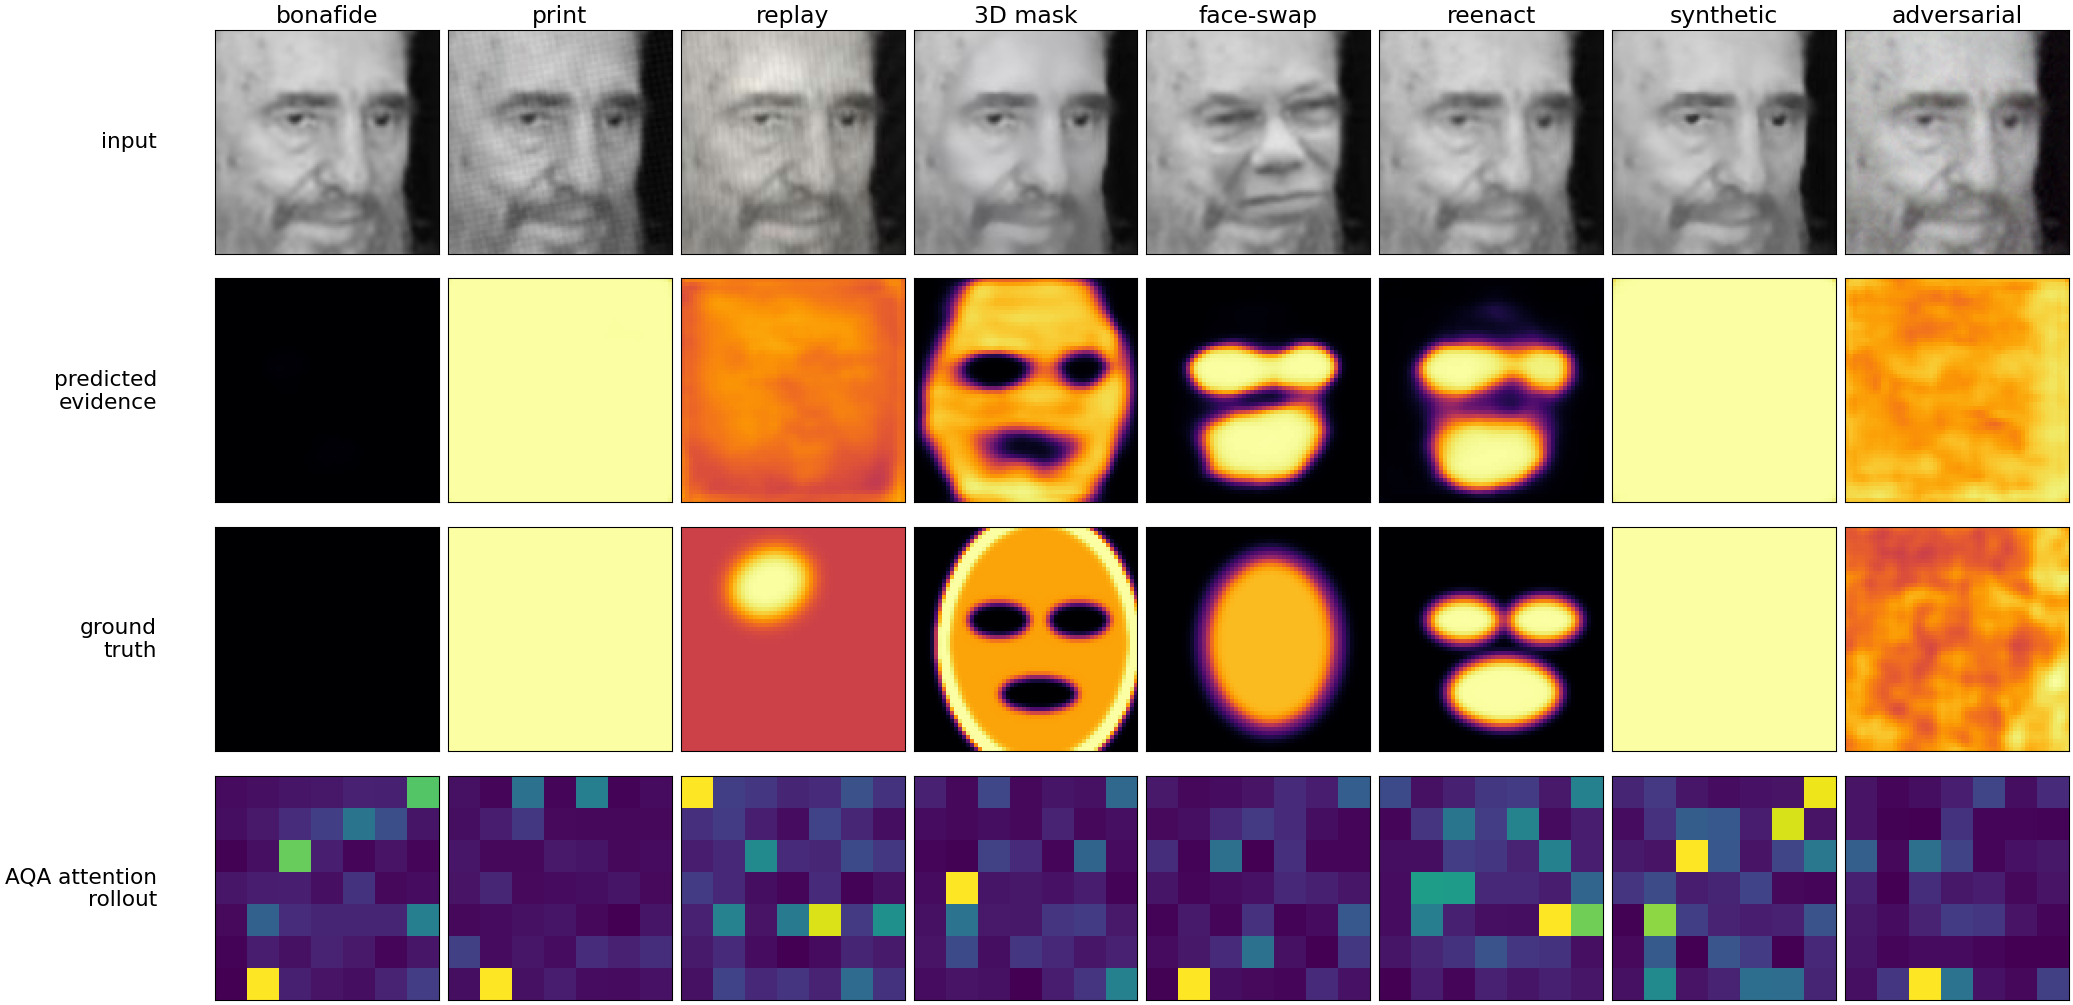
\includegraphics[width=\linewidth]{figures/qualitative.png}
\caption{One sample per family. Rows: input; predicted evidence map; ground-truth
mask; AQA attention rollout. The localiser recovers the eye/mouth support of the
reenactment, the cut-outs of the 3-D mask, and spreads over the whole frame for
print, synthetic and adversarial. It is not perfect: on this face-swap it predicts
an eye/mouth pattern resembling reenactment rather than the ground-truth blending
ellipse, and on replay it misses the localised glare spot.}
\label{fig:qual}
\end{figure}

\begin{figure}[t]
\centering
\fbox{\parbox{0.95\linewidth}{\ttfamily\footnotesize
\raggedright
Attack: Replay attack \\
Confidence: 98\% \\
Risk: Medium \\[4pt]
The sample is classified as a replay attack (physical presentation attack) with 98\% posterior probability; the probability that it is an attack of any kind is 99.7\%. That class is characterised by a sub-pixel display lattice aliasing into a moire beat, together with specular backlight glare and reduced dynamic range. Evidence is concentrated in the forehead (mean response 0.75), followed by eye region, nose / midface; it covers 100\% of the crop with a spatial dispersion of 1.00. The dominant quantum evidence mode is \#1, whose learned selectivity is highest for 'replay' (activation 0.074), corroborating the class decision. Vacuity is low (0.04): the evidence is strong and consistent with a single known family. The adaptive attention gate settled at 0.23, i.e. 23\% of the attention score came from the Born (interference) channel rather than the classical dot product. Recommended action: reject (risk score 0.71 -> Medium).

}}
\caption{A verdict as printed by the deployed system. Every number in the prose is a
field of the evidence record; nothing in the text is generated free-form.}
\label{fig:report}
\end{figure}

% =====================================================================
\section{The Research Gap, Revisited}\label{sec:gap}
% =====================================================================
We restate the gap from Section~\ref{sec:related} as five concrete deficits, and pair
each one with the mechanism that addresses it and the measurement that shows the
effect.

\textbf{Gap 1: detection is unified only in-distribution.} The unified corpora
\cite{yu2024unified,ma2025uniattackplus} show near-saturated seen-attack numbers next
to $22$ to $44\%$ ACER once attack families are withheld. Nothing in those
architectures represents ``this belongs to no family I know'', because a softmax has
to put all of its mass somewhere. \emph{Mechanism:} the Dirichlet evidential head
makes total evidence, and therefore vacuity, an explicit output, and PUES trains that
output against an outlier proxy built from the attack taxonomy itself rather than an
unrelated image pool. \emph{Evidence:} the unseen-family detection rate and novelty
AUROC in Table~\ref{tab:loao}, and the w/o-PUES row of Table~\ref{tab:oablate}.

\textbf{Gap 2: attention is linear, but much of the evidence is interference.}
Moir\'e beats, halftone screens, and upsampling checkerboards are periodic structures
whose sign carries no information. A dot-product score is sign-sensitive and has to
spend capacity learning that invariance from scratch. \emph{Mechanism:} the Born
channel scores token pairs by a squared overlap, which is sign-invariant by
construction, and the input-conditioned gate recruits it only where it helps.
\emph{Evidence:} the w/o-AQA rows of Tables~\ref{tab:abl} and~\ref{tab:oablate}, and
the per-family gate values in Table~\ref{tab:gates}. We should be careful about what
the gate table does and does not show. It confirms the channel is genuinely used,
with a mean around $0.31$ and a clear per-family structure, and the ablation confirms
it contributes. It does \emph{not} confirm our original hypothesis that the gate
would open furthest on the most periodic families. Print and adversarial open widest,
while replay, the family with the most obvious moir\'e beat, opens least. The
mechanism works; our story about why it works is not settled by this measurement.

\textbf{Gap 3: pixel supervision targets a liveness proxy, not the evidence itself.}
Depth maps \cite{liu2018auxiliary,yu2021revisiting} are undefined for a digitally
manipulated but physically genuine capture, so a unified detector built on them
inherits a supervision signal that is meaningless for half of its own label space.
\emph{Mechanism:} we supervise the actual injected support directly, which our
benchmark can provide because it knows exactly where it wrote the evidence.
\emph{Evidence:} Table~\ref{tab:loc}'s region-level IoU on families for which a depth
target would carry zero information, and Fig.~\ref{fig:qual}.

\textbf{Gap 4: MLLM explanations are post-hoc narration.} FFAA \cite{huang2024ffaa}
and M2F2-Det \cite{guo2025m2f2det} give the language model the raw image, not the
detector's internal state, so the narrative is unverifiable and can contradict the
decision it is meant to explain. \emph{Mechanism:} we invert the dependency. The
forward pass emits a typed evidence record, and language is realised from that record
alone, with the optional hosted back-end constrained and then re-verified against the
same record. \emph{Evidence:} the localisation channel of Table~\ref{tab:faith} is
the one quoted in the generated text (Fig.~\ref{fig:report}), and it is also a channel
that clears the random control on deletion. The grounded realiser's hallucination
rate is zero by construction.

\textbf{Gap 5: a score is not a decision.} An operator has to act on something, and a
scalar in $[0,1]$ with no calibrated meaning and no severity model does not tell them
what to do. \emph{Mechanism:} the risk calibrator converts posterior, vacuity and
evidence area into a bounded risk score with an explicit unknown-attack premium, so
that a confidently-unknown sample is escalated to human review instead of silently
passing through. \emph{Evidence:} the verdict of Fig.~\ref{fig:report} shows the
mechanism working on a single sample. We do \emph{not} yet have evidence that the
$u\ge0.55$ referral rule helps on unseen attacks. In every leave-one-attack-out
fold, genuine faces receive at least as much mean vacuity as the held-out family
($0.54$, $0.37$, $0.42$, $0.58$ against $0.54$, $0.31$, $0.43$, $0.39$), so the rule
as set is likely to refer at least as many genuine faces as unseen attacks. Setting
the referral threshold, and measuring its referral rates per group, is left to
future work (Section~\ref{sec:limits}).

% =====================================================================
\section{Limitations}\label{sec:limits}
% =====================================================================
We would rather state these plainly than let a reader discover them.

\textbf{Simulated evidence.} Our operators are models of physical and generative
processes, not the processes themselves. They reproduce the artifact families the
forensic literature has identified as discriminative, including halftone, moir\'e,
sub-pixel lattice, blending boundary, resolution mismatch, checkerboard, spectral
peak and gradient perturbation, but the joint statistics of a real re-capture are
richer than any operator we can write down. Absolute numbers in this paper should not
be compared directly against numbers reported on captured corpora. The comparisons
that are valid are the ones made \emph{inside} this paper, where every method sees
identical data.

\textbf{No external validation.} Every number reported here comes from our own
simulated benchmark. We release adapters that map the identical taxonomy, protocols
and model code onto seven public capture-based corpora, and those adapters are
regression-tested against synthetic fixtures that replicate each corpus's on-disk
layout. They have not been run on the real corpora. Nothing in this paper should be
read as validation on captured data, and we would ask reviewers and readers to treat
the released configurations as an invitation to replicate rather than as evidence
that replication has already happened.

\textbf{Single seed.} Every number here comes from one run at seed $0$. The paired
significance tests establish that the closed-set differences are not sampling noise
\emph{for this seed}, but they say nothing about initialisation variance, and the
leave-one-attack-out margins in particular, several of which are within a few points,
deserve repeats before they are leaned on.

\textbf{Reduced budget for leave-one-attack-out.} P2 models are trained for $5$
epochs on $4{,}382$ samples, P1 models for $10$ epochs on $19{,}200$. Models are
compared fairly within each protocol, but P1 and P2 numbers are not comparable with
each other, and the drop from P1 to P2 mixes the effect of the held-out family with
the effect of the smaller budget. A P2 run at the full P1 budget, or a matched
reduced-budget P1 run, is needed to separate them.

\textbf{Referral rule not validated.} The $u\ge0.55$ threshold that sends a sample
to human review was set by hand. Under leave-one-attack-out, genuine faces carry
as much vacuity as unseen attacks on average, so this rule is unlikely to separate
them. Its per-group referral rates were not measured, because per-sample outputs of
the leave-one-attack-out runs were not kept.

\textbf{Grayscale source imagery.} Domain A is grayscale, which removes colour cues
equally for every method and makes the task harder rather than easier. It does mean
the colour-domain components of our print and replay operators are inactive there.
Domain B is what exercises them.

\textbf{Still images only.} Temporal evidence, meaning rPPG, blink dynamics, and the
frame-to-frame refresh beat of a replay attack, is entirely out of scope. The
architecture would extend fairly naturally by treating a short clip as a token
sequence, and the Born channel seems well suited in principle to the temporal
periodicity of a refresh beat, but we have not evaluated that extension.

\textbf{Localisation threshold and sampling.} Predicted evidence maps are binarised
at a fixed $0.5$. That is a convention rather than a policy, it was never fitted on
validation or anywhere else, and it is applied identically across methods.
Separately, localisation metrics are computed over the first $600$ test samples in
dataset order, and the pixel-level AUC over a $200$-sample subset of those. On this
benchmark the sample is balanced, because the eight families interleave every eight
samples by construction, but on a corpus whose ordering groups samples by family that
sampling would be biased. Anyone porting this evaluation to another corpus should
stratify it.

\textbf{Ground-truth mask decoding.} For corpora that ship annotation videos rather
than generator masks, our adapter binarises the decoded annotation at $0.15$. That
value affects no number in this paper, since every family in our own benchmark
carries an exact operator mask, but it governs any future run on a real corpus and it
has not been validated against real annotations. Relatedly, where a corpus ships no
mask at all, our adapter substitutes a smoothed face-region ellipse as a proxy
target, and that proxy is not currently excluded from IoU reporting. Neither
condition is triggered by any result here, but both would need handling before an
external localisation number could be trusted.

\textbf{Compute scale.} Every experiment here runs on CPU with a $1.3$M-parameter
model. The public challenge results \cite{ma2025uniattackplus} make clear that large
pretrained multimodal backbones are currently the strongest known unified detectors.
Our contributions are orthogonal to backbone scale, since AQA is a drop-in attention
mechanism and the evidential head, PUES, the localiser and the reasoning module can
all attach to any encoder. Combining them with a LoRA-adapted large vision-language
backbone is a natural next step and a substantially larger undertaking than this
paper.

\textbf{White-box adaptive adversaries.} Our adversarial class is a transfer attack,
crafted against a surrogate that shares no weights with any evaluated model. A
white-box adversary with actual gradient access to X-UAD itself, including through
the vacuity channel, is a meaningfully stronger threat model and is not evaluated
here.

% =====================================================================
\section{Directions We Think Are Genuinely Open}\label{sec:open}
% =====================================================================
A few of the questions below go beyond what this paper set out to do, and we name
them explicitly rather than folding them into the limitations list, because we are
not aware of existing work in this space that has tackled them yet.

\textbf{Attacking the uncertainty channel itself.} Almost all open-set and
evidential work, ours included, evaluates robustness of the \emph{class decision}
under adversarial pressure. Very little evaluates whether the \emph{vacuity signal}
itself can be attacked independently. Because our vacuity head reads a stop-gradient
copy of the shared representation, an adversary with white-box access could plausibly
search for a perturbation that lowers $u$, manufacturing false confidence, while
barely moving the class logits at all, since the two objectives are explicitly
decoupled during training. Whether that decoupling, which is exactly what makes the
uncertainty channel free with respect to accuracy, also makes it a uniquely soft
target is, as far as we can tell, an open question.

\textbf{PUES beyond pairwise blends.} We only ever mix two attack families at a time.
Whether three-way or higher-order mixtures, or mixtures weighted by how forensically
\emph{similar} two families already are rather than a flat $\mathrm{Beta}(2,2)$,
produce a better outlier proxy is untested. There is a plausible argument either way.
Closer families might produce a harder and more informative training signal for the
vacuity boundary, or they might produce blends that are accidentally too close to a
real attack and corrupt the class-direction gradient.

\textbf{A learned, rather than fixed, risk policy.} Section~\ref{sec:method}
deliberately keeps the risk calibrator's coefficients unlearned, for auditability
reasons we still believe in. But nothing stops a clearly-labelled meta-model from
learning site-specific coefficients from a small amount of labelled operator
feedback, such as analyst overrides of the band, while leaving the underlying
detector and its explanation completely untouched. That would let a deployment site's
risk tolerance adapt over time without ever touching the part of the system
responsible for the actual forensic decision.

\textbf{Cross-domain shift and attack-family shift as a joint problem.} Every
domain-generalisation technique for face anti-spoofing we are aware of
\cite{wang2022ssan,shao2019mada,jia2020ssdg} targets capture-domain shift alone,
using only \emph{seen} attack families. Every open-set technique, including PUES,
targets attack-family shift on a \emph{single} capture domain. What happens at the
intersection, where an unseen attack family arrives through an unseen capture domain
simultaneously, has not been studied. Our own Table~\ref{tab:cross} suggests the joint
case may not simply be the product of the two individual failure rates. Closing this
gap would need a benchmark explicitly designed to vary both axes independently, which
our generator is well placed to provide.

\textbf{Explanation faithfulness under distribution shift.} Table~\ref{tab:faith}
measures faithfulness only on in-distribution, seen-attack samples. Whether an
intrinsic explanation stays faithful when the underlying detector is operating in the
P2 or P3 regime, which is to say whether the localisation map still points at
something real when the class decision itself is unreliable, is untested here. A
model that is uncertain but still produces a confident-looking localisation map would
be a genuinely dangerous failure mode for exactly the auditability reasons this paper
cares about.

% =====================================================================
\section{Conclusion}
% =====================================================================
X-UAD detects physical and digital face attacks with a single model, reports how much
it does not know, shows where the evidence sits, and explains itself in language that
can be audited sentence by sentence. Three ideas make this combination possible: a
Born-rule attention channel that matches the interference character of the underlying
evidence at a parameter cost of $\mathcal{O}(dL)$; an orthonormal quantum evidence
basis that serves simultaneously as a classification feature and as the explanation
itself; and pseudo-unseen evidence suppression, which manufactures an out-of-taxonomy
proxy directly from the attack taxonomy and turns Dirichlet vacuity into a usable
open-set score.

The gains concentrate on unseen attack families, calibration and localisation, rather
than on the already-saturated seen-attack task. The costs are real and we have
reported them: a $0.75$ ACER point deficit against the strongest baseline on P1, a
mildly inverted uncertainty ranking on the adversarial fold, an insertion-faithfulness
result that does not clear its control, and a cross-domain protocol on which no
method in this paper, ours included, performs acceptably. Every number here comes from
a single seed on a simulated benchmark, and validating these mechanisms on captured
corpora, with repeated seeds, is the necessary next step rather than an optional one.

\section*{Acknowledgment}
The source faces used to build the benchmark are drawn from the Labeled Faces in the
Wild database \cite{huang2007lfw}, used under its terms for non-commercial research.

\bibliographystyle{IEEEtran}
\bibliography{refs}

\end{document}
